%  LaTeX support: latex@mdpi.com 
%  For support, please attach all files needed for compiling as well as the log file, and specify your operating system, LaTeX version, and LaTeX editor.

%=================================================================
\documentclass[electronics,article,submit,pdftex,moreauthors]{Definitions/mdpi} 
%\documentclass[preprints,article,submit,pdftex,moreauthors]{Definitions/mdpi} 
% For posting an early version of this manuscript as a preprint, you may use "preprints" as the journal. Changing "submit" to "accept" before posting will remove line numbers.

%--------------------
% Class Options:
%--------------------
%----------
% journal
%----------
% Choose between the following MDPI journals:
% accountaudit, acoustics, actuators, addictions, adhesives, adolescents, aerobiology, aerospace, agriculture, agriengineering, agrochemicals, agronomy, ai, aichem, aieng, aimater, aimed, aipa, air, aisens, algorithms, allergies, alloys, amh, analog, analytica, analytics, anatomia, anesthres, animals, antibiotics, antibodies, antioxidants, applbiosci, appliedchem, appliedmath, appliedphys, applmech, applmicrobiol, applnano, applsci, aquacj, architecture, arm, arthropoda, asc, asi, astronautics, astronomy, atmosphere, atoms, audiolres, automation, axioms, bacteria, batteries, bdcc, beverages, biochem, bioengineering, biologics, biology, biomass, biomechanics, biomed, biomedicines, biomedinformatics, biomimetics, biomolecules, biophysica, bioresourbioprod, biosensors, biosphere, biotech, birds, blockchains, bloods, blsf, brainsci, breath, buildings, cancers, carbon, cardio, cardiogenetics, cardiovascmed, catalysts, cells, ceramics, challenges, chemengineering, chemistry, chemosensors, chemproc, children, chips, cimb, civileng, cleantechnol, climate, clinbioenerg, clinpract, clockssleep, cmd, cmtr, coasts, coatings, colloids, colorants, commodities, complexities, complications, compounds, computation, computers, condensedmatter, conservation, constrmater, cosmetics, covid, crops, cryo, cryptography, crystals, csmf, ctn, culture, curroncol, cyber, dairy, data, ddc, dentistry, dermato, dermatopathology, designs, devices, dhi, diabetology, diagnostics, dietetics, digital, disabilities, diseases, diversity, dna, drones, dynamics, earth, ebj, ecm, ecologies, edm, eesp, electricity, electrochem, electronicmat, electronics, encyclopedia, endocrines, energies, eng, engproc, entomology, entropy, environments, environremediat, epidemiologia, epigenomes, esa, est, fermentation, fibers, fintech, fire, fishes, fluids, foods, forecasting, forensicsci, forests, fossstud, foundations, fractalfract, fuels, future, futureinternet, futurepharmacol, futurephys, futuretransp, galaxies, gases, gastroent, gastrointestdisord, gastronomy, gels, genes, geographies, geohazards, geomatics, geometry, geosciences, geotechnics, geriatrics, germs, glacies, grasses, green, greenhealth, gucdd, hardware, hazardousmatters, healthcare, hearts, hemato, hematolrep, hep, heritage, higheredu, highthroughput, horticulturae, hospitals, hydrobiology, hydrogen, hydrology, hydropower, hygiene, idr, iic, ijem, ijerph, ijgi, ijmd, ijms, ijns, ijom, ijpb, ijt, ijtm, ijtpp, ime, immuno, informatics, information, infrastructures, inorganics, insects, instruments, inventions, iot, j, jaestheticmed, jal, jcdd, jcm, jcp, jcrm, jcs, jcto, jdad, jdb, jdream, jemr, jeta, jfb, jfmk, jgbg, jgg, jimaging, jlpea, jmahp, jmmp, jmms, jmp, jmse, jne, jnt, jof, joi, joitmc, joma, jop, joptm, jor, jox, jpbi, jphytomed, jpm, jsan, jtaer, jvd, jzbg, kidneydial, kinasesphosphatases, knowledge, labmed, laboratories, lae, land, life, lights, limnolrev, lipidology, liquids, livers, logics, logistics, lubricants, lymphatics, machines, macromol, magnetism, magnetochemistry, make, marinedrugs, materials, materproc, mathematics, mca, measurements, medicina, medicines, medsci, membranes, merits, metabolites, metals, meteorology, methane, metrics, metrology, micro, microarrays, microbiolres, microelectronics, micromachines, microorganisms, microplastics, microwave, minerals, mining, mmphys, modelling, molbank, molecules, mps, msf, mti, multimedia, muscles, nanoenergyadv, nanomanufacturing, nanomaterials, ncrna, ndt, network, neuroglia, neuroimaging, neurolint, neurosci, nitrogen, notspecified, nursrep, nutraceuticals, nutrients, obesities, occuphealth, oceans, ohbm, onco, optics, oral, organics, organoids, osteology, oxygen, pandemics, parasites, parasitologia, particles, pathogens, pathophysiology, pediatrrep, pets, pharmaceuticals, pharmaceutics, pharmacoepidemiology, pharmacy, philosophies, photochem, photonics, phycology, physchem, physics, physiologia, plants, plasma, platforms, pollutants, polymers, polysaccharides, populations, poultry, powders, precipitation, precisoncol, preprints, proceedings, processes, prosthesis, proteomes, psf, psychiatryint, psychoactives, purification, quantumrep, quaternary, qubs, radiation, rdt, reactions, realestate, receptors, recycling, regeneration, remotesensing, reports, reprodmed, resources, rheumato, rjpm, robotics, rsee, ruminants, safety, sci, scipharm, sclerosis, seeds, sensors, separations, sexes, shi, signals, sinusitis, siuj, skins, smartcities, sna, societies, software, soilsystems, solar, solids, spectroscj, sports, standards, stats, std, stratsediment, stresses, surfaces, surgeries, suschem, sustainability, symmetry, synbio, systems, tae, targets, taxonomy, technologies, telecom, test, textiles, thalassrep, therapeutics, thermo, timespace, tomography, toxics, toxins, tph, transplantology, transportation, traumacare, traumas, tri, tropicalmed, universe, urbansci, uro, vaccines, vehicles, venereology, vetsci, vibration, virtualworlds, viruses, vision, waste, water, welding, wem, wevj, wild, wind, women, world, zoonoticdis

%---------
% article
%---------
% The default type of manuscript is "article", but can be replaced by: 
% abstract, addendum, article, benchmark, book, bookreview, briefcommunication, briefreport, casereport, changes, clinicopathologicalchallenge, comment, commentary, communication, conceptpaper, conferenceproceedings, correction, conferencereport, creative, datadescriptor, discussion, entry, expressionofconcern, extendedabstract, editorial, essay, erratum, fieldguide, hypothesis, interestingimages, letter, meetingreport, monograph, newbookreceived, obituary, opinion, proceedingpaper, projectreport, reply, retraction, review, perspective, protocol, shortnote, studyprotocol, supfile, systematicreview, technicalnote, viewpoint, guidelines, registeredreport, tutorial,  giantsinurology, urologyaroundtheworld
% supfile = supplementary materials

%----------
% submit
%----------
% The class option "submit" will be changed to "accept" by the Editorial Office when the paper is accepted. This will only make changes to the frontpage (e.g., the logo of the journal will get visible), the headings, and the copyright information. Also, line numbering will be removed. Journal info and pagination for accepted papers will also be assigned by the Editorial Office.

%------------------
% moreauthors
%------------------
% If there is only one author the class option oneauthor should be used. Otherwise use the class option moreauthors.

%---------
% pdftex
%---------
% The option pdftex is for use with pdfLaTeX. Remove "pdftex" for (1) compiling with LaTeX & dvi2pdf (if eps figures are used) or for (2) compiling with XeLaTeX.

%=================================================================
% MDPI internal commands - do not modify
\firstpage{1} 
\makeatletter 
\setcounter{page}{\@firstpage} 
\makeatother
\pubvolume{1}
\issuenum{1}
\articlenumber{0}
\pubyear{2026}
\copyrightyear{2026}
%\externaleditor{Firstname Lastname} % More than 1 editor, please add `` and '' before the last editor name
\datereceived{ } 
\daterevised{ } % Comment out if no revised date
\dateaccepted{ } 
\datepublished{ } 
%\datecorrected{} % For corrected papers: "Corrected: XXX" date in the original paper.
%\dateretracted{} % For retracted papers: "Retracted: XXX" date in the original paper.
%\doinum{} % Used for some special journals, like molbank
%\pdfoutput=1 % Uncommented for upload to arXiv.org
%\CorrStatement{yes}  % For updates
%\longauthorlist{yes} % For many authors that exceed the left citation part
%\IsAssociation{yes} % For association journals

%=================================================================
% Add packages and commands here. The following packages are loaded in our class file: fontenc, inputenc, calc, indentfirst, fancyhdr, graphicx, epstopdf, lastpage, ifthen, float, amsmath, amssymb, lineno, setspace, enumitem, mathpazo, booktabs, titlesec, etoolbox, tabto, xcolor, colortbl, soul, multirow, microtype, tikz, totcount, changepage, attrib, upgreek, array, tabularx, pbox, ragged2e, tocloft, marginnote, marginfix, enotez, amsthm, natbib, hyperref, cleveref, scrextend, url, geometry, newfloat, caption, draftwatermark, seqsplit
% cleveref: load \crefname definitions after \begin{document}

%=================================================================
% Please use the following mathematics environments: Theorem, Lemma, Corollary, Proposition, Characterization, Property, Problem, Example, ExamplesandDefinitions, Hypothesis, Remark, Definition, Notation, Assumption
%% For proofs, please use the proof environment (the amsthm package is loaded by the MDPI class).

%=================================================================
% Full title of the paper (Capitalized)
\Title{An Efficient Attention-Enhanced MobileNetV2 Framework for Plant Disease Detection on Resource-Constrained Devices}

% Author Orchid ID: enter ID or remove command
\newcommand{\orcidauthorA}{0009-0008-7624-2520}

% Authors, for the paper (add full first names)
\Author{Emmanuel Udoh $^{1}$\orcidA{}, Mohammed Ayoub Alaoui Mhamdi $^{1}$ and Madjid Allili $^{1}$}

%\longauthorlist{yes}

% MDPI internal command: Authors, for metadata in PDF
\AuthorNames{Emmanuel Udoh, Mohammed Ayoub Alaoui Mhamdi and Madjid Allili}

% Affiliations / Addresses (Add [1] after \address if there is only one affiliation.)
\address{
$^{1}$ Department of Computer Science, Bishop’s University, Sherbrooke, QC, Canada
}

% Contact information of the corresponding author
\corres{Correspondence: malaoui@ubishops.ca}

% Current address and/or shared authorship
%\firstnote{Current address: Affiliation.}  
% Current address should not be the same as any items in the Affiliation section.

%\secondnote{These authors contributed equally to this work.}
% The commands \thirdnote{} till \eighthnote{} are available for further notes.

%\simplesumm{} % Simple summary

%\conference{} % An extended version of a conference paper

% Abstract (Do not insert blank lines, i.e. \\) 
\abstract{Plant diseases motivate accurate and computationally efficient image-based diagnostic methods. This paper evaluates a framework that places a Convolutional Block Attention Module (CBAM) after the final MobileNetV2 convolutional feature map and before global average pooling. Experiments use 54,306 controlled-background PlantVillage images in 38 classes. In a consistent re-evaluation of the saved floating-point models, MobileNetV2 + CBAM achieved 97.17\% accuracy and 97.15\% weighted F1-score, compared with 96.78\% and 96.73\% for MobileNetV2. A paired evaluation of the converted models yielded a 0.64-percentage-point accuracy difference (95\% CI: 0.31--0.96; exact McNemar $p<0.001$). The proposed model contains 4.02 million parameters, requires 0.604 GFLOPs (approximately 0.302 GMACs), and produces a 4.07 MiB dynamic-range-quantized TensorFlow Lite file with 96.70\% accuracy. On an Intel i7-11800H CPU using TensorFlow Lite/XNNPACK with eight threads, median batch-one latency was 45.42 ms (P95: 102.54 ms), excluding preprocessing. Grad-CAM examples show lesion-focused behavior and shared failure cases. These results establish a compact accuracy--cost trade-off under the study conditions; field generalization, energy consumption, independent training runs, and target-device performance remain to be validated.}

% Keywords
\keyword{Plant disease detection; MobileNetV2; CBAM; lightweight deep learning; edge computing; TensorFlow Lite; precision agriculture}

% The fields PACS, MSC, and JEL may be left empty or commented out if not applicable
%\PACS{J0101}
%\MSC{}
%\JEL{}

%%%%%%%%%%%%%%%%%%%%%%%%%%%%%%%%%%%%%%%%%%
% Only for the journal Diversity
%\LSID{\url{http://}}

%%%%%%%%%%%%%%%%%%%%%%%%%%%%%%%%%%%%%%%%%%
% Only for the journal Applied Sciences
%\featuredapplication{Authors are encouraged to provide a concise description of the specific application or a potential application of the work. This section is not mandatory.}
%%%%%%%%%%%%%%%%%%%%%%%%%%%%%%%%%%%%%%%%%%

%%%%%%%%%%%%%%%%%%%%%%%%%%%%%%%%%%%%%%%%%%
% Only for the journal Data
%\dataset{DOI number or link to the deposited data set if the data set is published separately. If the data set shall be published as a supplement to this paper, this field will be filled by the journal editors. In this case, please submit the data set as a supplement.}
%\datasetlicense{License under which the data set is made available (CC0, CC-BY, CC-BY-SA, CC-BY-NC, etc.)}

%%%%%%%%%%%%%%%%%%%%%%%%%%%%%%%%%%%%%%%%%%
% Only for the journal BioTech, Fishes, Neuroimaging and Toxins
%\keycontribution{The breakthroughs or highlights of the manuscript. Authors can write one or two sentences to describe the most important part of the paper.}

%%%%%%%%%%%%%%%%%%%%%%%%%%%%%%%%%%%%%%%%%%
% Only for the journal Encyclopedia
%\encyclopediadef{For entry manuscripts only: please provide a brief overview of the entry title instead of an abstract.}

%%%%%%%%%%%%%%%%%%%%%%%%%%%%%%%%%%%%%%%%%%
% Different journals have different requirements. Please check the specific journal guidelines in the "Instructions for Authors" on the journal's official website.
%\addhighlights{yes}
%\renewcommand{\addhighlights}{%
%
%\noindent The goal is to increase the discoverability and readability of the article via search engines and other scholars. Highlights should not be a copy of the abstract, but a simple text allowing the reader to quickly and simplified find out what the article is about and what can be cited from it. Each of these parts should be devoted up to 2~bullet points.\vspace{3pt}\\
%\textbf{What are the main findings?}
% \begin{itemize}[labelsep=2.5mm,topsep=-3pt]
% \item First bullet.
% \item Second bullet.
% \end{itemize}\vspace{3pt}
%\textbf{What are the implications of the main findings?}
% \begin{itemize}[labelsep=2.5mm,topsep=-3pt]
% \item First bullet.
% \item Second bullet.
% \end{itemize}
%}

%%%%%%%%%%%%%%%%%%%%%%%%%%%%%%%%%%%%%%%%%%
\begin{document}

%%%%%%%%%%%%%%%%%%%%%%%%%%%%%%%%%%%%%%%%%%
\section{Introduction}

Plant diseases remain a major threat to global agricultural productivity, food security, and economic stability. Since many disease symptoms first appear on plant leaves, visual inspection is commonly used for early diagnosis. However, manual inspection is often time-consuming, subjective, and dependent on expert availability, particularly in rural or resource-constrained agricultural environments. Delayed or inaccurate diagnosis may lead to crop losses, inappropriate treatment, and unnecessary pesticide use. Therefore, accurate, scalable, and accessible plant disease detection systems are important for precision agriculture.

Recent advances in deep learning have significantly improved image-based plant disease classification. Convolutional neural networks (CNNs) can automatically learn discriminative visual features from leaf images, reducing the dependence on handcrafted feature extraction. Publicly available datasets such as PlantVillage have further supported the development and benchmarking of deep learning models for plant disease recognition~\cite{mohanty2016,hughes2015open}. Nevertheless, many high-performing CNN architectures require large numbers of parameters and computationally expensive operations, limiting their practical use on mobile phones, embedded systems, and other resource-constrained devices.

Lightweight architectures such as MobileNetV2 address this limitation by reducing computational complexity while maintaining competitive performance. MobileNetV2 uses inverted residual blocks and depthwise separable convolutions to reduce the number of operations required for feature extraction~\cite{sandler2018mobilenetv2}. However, lightweight models may have lower representational capacity than deeper architectures. Attention mechanisms offer a promising strategy for improving feature representation with modest additional computational cost. In particular, the Convolutional Block Attention Module (CBAM) applies sequential channel and spatial attention to emphasize informative feature responses while suppressing less relevant information~\cite{woo2018cbam}. This makes CBAM suitable for enhancing lightweight CNNs used in plant disease detection.

This paper evaluates an attention-enhanced MobileNetV2 framework as a candidate for resource-constrained plant disease classification. CBAM is integrated after the final MobileNetV2 convolutional feature map and before global average pooling. The study does not claim that combining two established components is itself a new attention mechanism. Instead, its contribution is an explicitly defined late-attention configuration and an empirical analysis of the accuracy--cost trade-off under a common transfer-learning protocol. The model is evaluated on PlantVillage against MobileNetV2, InceptionV3, and Xception using classification and computational proxy metrics. Because PlantVillage uses controlled backgrounds and latency was not measured on a target edge device, the evaluation is evidence of compactness rather than proof of field or real-time deployment readiness.

The main contributions of this paper are summarized as follows:

\begin{itemize}
    \item A reproducible late-attention configuration is specified by placing CBAM once, after MobileNetV2's final convolutional feature map and before global average pooling.
    
    \item The incremental effect of this configuration is quantified against an otherwise comparable MobileNetV2 baseline.
    
    \item A comparative evaluation is conducted against MobileNetV2, InceptionV3, and Xception using standard classification metrics on the PlantVillage dataset.
    
    \item The study reports parameter count, FLOPs/MACs, serialized model size, dynamic-range TFLite accuracy, and a reproducible laptop-CPU latency protocol, while separating this evidence from target-device claims.
    
    \item The limitations imposed by controlled-background data, a single training run, partially fine-tuned backbones, legacy generator subsampling, audited cross-split duplicates, and the absence of field-device and energy measurements are identified to delimit the conclusions.
\end{itemize}

The remainder of this paper is organized as follows. Section~2 reviews related work on plant disease detection, lightweight CNN architectures, and attention mechanisms. Section~3 presents the proposed MobileNetV2 + CBAM framework. Section~4 describes the experimental setup, results, discussion, and deployment-oriented computational analysis. Finally, Section~5 concludes the paper and outlines future research directions.


%%%%%%%%%%%%%%%%%%%%%%%%%%%%%%%%%%%%%%%%%%
\section{Related Work}

Plant disease detection has evolved from traditional image processing and handcrafted feature-based methods toward deep learning-based approaches. Earlier computer vision techniques typically relied on preprocessing, segmentation, color or texture feature extraction, and machine learning classifiers. Barbedo~\cite{barbedo2013} reviewed digital image processing methods for detecting and classifying plant diseases, while Zhang et al.~\cite{zhang2014} discussed the use of computer vision in plant pathology. Although these methods demonstrated the feasibility of automated disease diagnosis, their reliance on handcrafted features and controlled imaging conditions limited their robustness across different crops, disease symptoms, and environmental variations. With the availability of plant disease image datasets, convolutional neural networks (CNNs) became widely adopted for automated feature learning. Mohanty et al.~\cite{mohanty2016} demonstrated the effectiveness of deep learning on the PlantVillage dataset, while Sladojevic et al.~\cite{sladojevic2016} and Ferentinos~\cite{ferentinos2018} further showed that CNN-based models can achieve strong performance in plant disease classification. However, many high-performing CNNs are computationally demanding, which creates challenges for mobile and resource-constrained deployment.

Recent research has increasingly focused on lightweight CNN architectures to reduce computational complexity while maintaining competitive classification performance. MobileNet introduced depthwise separable convolutions as an efficient alternative to standard convolutional operations~\cite{howard2017mobilenets}, and MobileNetV2 further improved this design using inverted residual blocks and linear bottlenecks~\cite{sandler2018mobilenetv2}. Other architectures, such as InceptionV3~\cite{szegedy2016rethinking}, Xception~\cite{chollet2017xception}, and EfficientNet~\cite{tan2019efficientnet}, have also contributed to efficient CNN design, although they differ significantly in model size, parameter count, and deployment suitability. In plant disease detection, practical systems must consider not only accuracy but also inference time, memory requirements, and model size. Khan et al.~\cite{khan2023edge} investigated plant disease detection for edge computing devices and emphasized the importance of optimization and quantization for resource-constrained platforms. Similarly, Duhan et al.~\cite{duhan2025rtr} proposed RTR\_Lite\_MobileNetV2, an enhanced lightweight MobileNetV2-based model for plant disease detection and classification, showing the growing interest in MobileNetV2 variants for efficient agricultural diagnosis. Li et al.~\cite{li2024tea_mobilenetv2} also improved MobileNetV2 for tea leaf disease identification using Coordinate Attention, multi-branch convolution, and model compression, further supporting the relevance of lightweight CNNs for field-oriented applications.

Attention mechanisms have become an important strategy for improving CNN feature representation without necessarily replacing lightweight backbones with heavier architectures. The squeeze-and-excitation network introduced channel-wise feature recalibration~\cite{hu2018senet}, while the Convolutional Block Attention Module (CBAM) extended this idea by sequentially applying channel and spatial attention~\cite{woo2018cbam}. This is particularly relevant for plant disease recognition because symptoms often appear as localized spots, discoloration, or texture irregularities on leaf surfaces. Recent attention-based studies have further shown the usefulness of attention mechanisms in agricultural image analysis. Subburaj et al.~\cite{subburaj2025plantention} proposed Plantention, a lightweight attention-based model using a MobileNetV2 encoder for multi-crop leaf disease classification. Wen et al.~\cite{wen2025mnasnet} introduced a lightweight CNN for tea leaf disease and pest recognition and compared several attention mechanisms, including CA, ECA, SE, and CBAM. Pal et al.~\cite{pal2025mobres} proposed a lightweight and explainable CNN model for plant disease diagnosis and used interpretability techniques such as Grad-CAM, Grad-CAM++, and LIME to analyze model predictions. These studies indicate that attention-enhanced lightweight CNNs are becoming increasingly important for accurate, interpretable, and deployment-aware plant disease detection.

Despite these advances, many plant disease detection studies still emphasize classification accuracy more strongly than deployment-oriented evaluation. Recent review studies note that practical plant disease recognition systems must address challenges such as variable illumination, symptom similarity, overfitting, dataset bias, limited generalization, and real-world deployment constraints~\cite{zhao2025review,nyawose2025review,sajitha2024review}. In particular, fewer studies jointly analyze classification metrics such as accuracy, precision, recall, F1-score, and AUC together with computational indicators such as parameter count, model size, TensorFlow Lite size, and inference latency. This creates a gap between high-performing laboratory models and practical mobile or edge-based agricultural diagnostic systems. To examine this trade-off, this paper evaluates CBAM after the final MobileNetV2 feature map and before global average pooling. The objective is to improve the baseline while retaining a compact candidate architecture; suitability for a particular resource-constrained device is not asserted without device-specific validation.

Table~\ref{tab:recent_lightweight_work} positions the present study against representative work published in 2024--2025. The comparison is qualitative because the studies use different datasets, splits, preprocessing, hardware, and reporting conventions; their accuracy and latency values should not be treated as a controlled leaderboard. Importantly, recent work already combines MobileNetV2 with attention or other lightweight refinements. The distinction of the present study is therefore the evaluated single late-CBAM placement and its measured incremental trade-off against an unmodified MobileNetV2 baseline, not the invention of an attention-enhanced MobileNet family.

\begin{table}[H]
\caption{Scope comparison with representative recent lightweight plant-disease studies.}
\label{tab:recent_lightweight_work}
\centering
\small
\begin{tabularx}{\textwidth}{p{2.8cm} p{4.3cm} X}
\toprule
\textbf{Study} & \textbf{Lightweight strategy} & \textbf{Scope and relation} \\
\midrule
Li et al. (2024)~\cite{li2024tea_mobilenetv2} & MobileNetV2, coordinate attention, multi-branch convolution, and compression & Tea-leaf evaluation; a broader modification using a different attention mechanism. \\
Duhan et al. (2025)~\cite{duhan2025rtr} & RTR\_Lite\_MobileNetV2 & Confirms that lightweight MobileNetV2 variants form an active, non-unique design family. \\
Subburaj et al. (2025)~\cite{subburaj2025plantention} & Attention model with a MobileNetV2 encoder & Multi-crop scope; this study instead isolates one late CBAM block. \\
Wen et al. (2025)~\cite{wen2025mnasnet} & Lightweight CNN comparing CA, ECA, SE, and CBAM & Provides an attention ablation that remains necessary here under one common protocol. \\
Pal et al. (2025)~\cite{pal2025mobres} & MobileNetV2 plus residual learning (3.51 M parameters) & Two datasets and Grad-CAM/Grad-CAM++/LIME; 99.47\% on PlantVillage, under a different protocol. \\
This study & One CBAM block after the final MobileNetV2 convolutional map & Reports an incremental accuracy--cost trade-off; device and interpretability evidence remain outstanding. \\
\bottomrule
\end{tabularx}
\normalsize
\end{table}


%%%%%%%%%%%%%%%%%%%%%%%%%%%%%%%%%%%%%%%%%%
\section{Proposed Method}

This section presents the evaluated attention-enhanced lightweight framework. The objective is to test whether a single late CBAM block can improve a partially fine-tuned MobileNetV2 feature extractor without a large increase in model size. Mobile and edge deployment are treated as intended use cases that require separate hardware validation.

\subsection{Dataset Preparation}

The experiments use 54,306 PlantVillage images in 38 classes. Each class was partitioned independently with \texttt{train\_test\_split}: 70\% for training and 30\% temporary data, followed by an equal division of the temporary data into validation and test sets. Both operations used \texttt{random\_state=42}. The resulting directories contain 37,998 training images (69.97\%), 8,146 validation images (15.00\%), and 8,162 test images (15.03\%). Because the archived training notebooks additionally specified \texttt{validation\_split=0.2}, the fitted generators used 30,416 images from the training directory and 1,614 images from the validation directory; the test generator used all 8,162 test images. This legacy configuration is reported explicitly rather than being described as an 80/10/10 split.

Training images were rescaled to $[0,1]$ and augmented with rotations up to $25^{\circ}$, horizontal and vertical shifts of 0.2, zoom of 0.2, shear of 0.15, brightness factors from 0.8 to 1.2, horizontal flipping, and nearest-neighbor filling. Test images were only rescaled. MobileNetV2, MobileNetV2 + CBAM, and Xception used $224 \times 224$ inputs; InceptionV3 used its trained $299 \times 299$ input. A SHA-256 audit found no repeated filenames but identified 10 exact-image duplicate groups crossing directory splits; seven test images duplicated an image in training or validation. A sensitivity analysis therefore reports results both on all 8,162 test images and after excluding these seven test duplicates. The controlled acquisition conditions of PlantVillage---typically isolated leaves and uniform backgrounds---remain a limitation for field generalization.

\subsection{Overview of the Proposed Framework}

The proposed framework follows a transfer learning-based classification pipeline. Preprocessed images are passed through an ImageNet-pretrained MobileNetV2 backbone, the resulting convolutional feature maps are refined by sequential channel and spatial attention, and global average pooling plus a softmax layer produces the class probabilities.

The general workflow of the proposed framework can be summarized as follows:

\begin{equation}
    X \rightarrow F_{\text{MobileNetV2}}(X) \rightarrow F_{\text{CBAM}} \rightarrow F_{\text{GAP}} \rightarrow \hat{y},
\end{equation}

where $X$ denotes the input leaf image, $F_{\text{MobileNetV2}}(X)$ represents the feature maps extracted by the MobileNetV2 backbone, $F_{\text{CBAM}}$ denotes the attention-refined feature representation, $F_{\text{GAP}}$ represents global average pooling, and $\hat{y}$ is the predicted class probability distribution.

\begin{figure}[H]
\centering
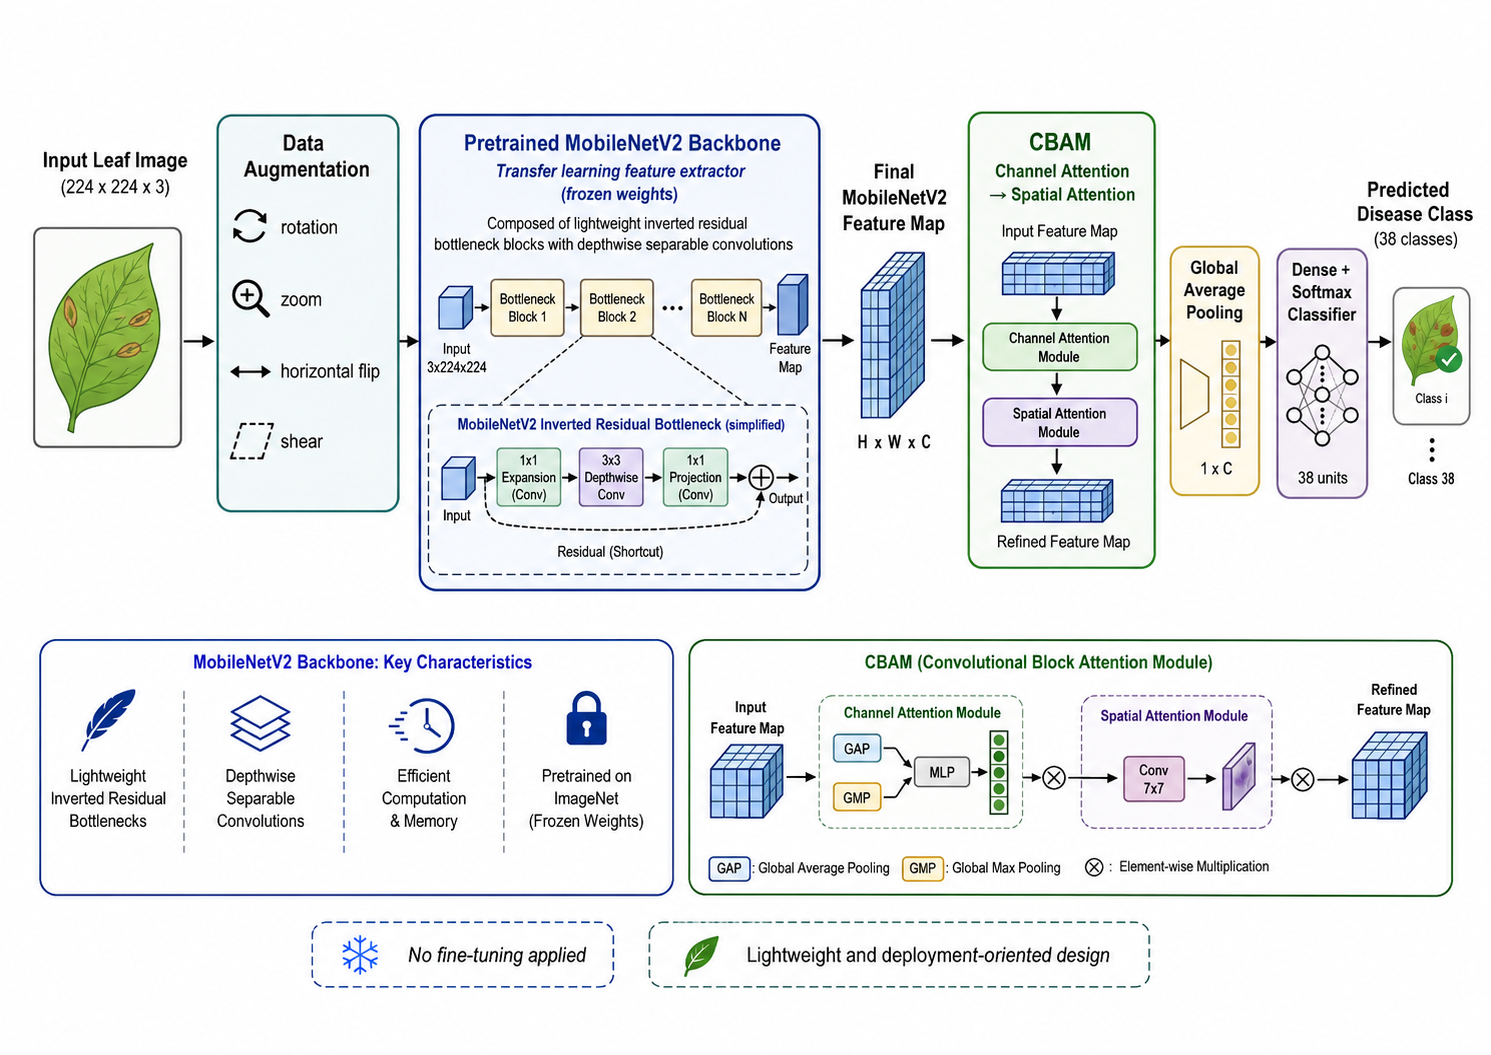
\includegraphics[width=0.95\textwidth]{figures/proposed_framework.png}
\caption{Overall architecture of the proposed attention-enhanced MobileNetV2 framework. CBAM is inserted after the final MobileNetV2 feature map and before global average pooling to refine channel and spatial feature representations.}
\label{fig:proposed_framework}
\end{figure}

\subsection{MobileNetV2 Backbone}

MobileNetV2 was selected because its inverted residual and linear-bottleneck design provides a well-established, readily convertible TensorFlow implementation with substantially fewer parameters than the heavier InceptionV3 and Xception comparators. This choice defines the present scope; it does not establish superiority over MobileNetV1, MobileNetV3, MobileNetV4, EfficientNet-B0, GhostNet, or ShuffleNetV2, which require a common-protocol comparison.

MobileNetV2 was selected as the baseline feature extraction architecture due to its lightweight design and suitability for mobile and embedded vision applications. Unlike conventional CNN architectures that rely heavily on standard convolutional operations, MobileNetV2 uses depthwise separable convolutions to reduce computational cost. A standard convolution applies filters across both spatial and channel dimensions simultaneously. In contrast, depthwise separable convolution decomposes this operation into a depthwise convolution followed by a pointwise convolution.

Given an input feature map, a standard convolution operation can be expressed as:

\begin{equation}
    Y = K * X,
\end{equation}

where $X$ is the input feature map, $K$ is the convolution kernel, $*$ denotes the convolution operation, and $Y$ is the output feature map.

In depthwise separable convolution, the depthwise convolution applies one spatial filter to each input channel independently:

\begin{equation}
    Y_{d}^{c} = K_{d}^{c} * X^{c},
\end{equation}

where $X^{c}$ is the $c$-th input channel, $K_{d}^{c}$ is the corresponding depthwise convolution kernel, and $Y_{d}^{c}$ is the resulting feature map for that channel. A pointwise convolution using $1 \times 1$ kernels is then applied to combine information across channels:

\begin{equation}
    Y = K_{p} * Y_{d},
\end{equation}

where $K_{p}$ represents the pointwise convolution kernel and $Y_{d}$ denotes the output of the depthwise convolution operation.

MobileNetV2 further improves efficiency through inverted residual blocks and linear bottlenecks~\cite{sandler2018mobilenetv2}. In an inverted residual block, the input feature representation is first expanded to a higher-dimensional space, processed using depthwise convolution, and then projected back to a lower-dimensional representation. The use of linear bottlenecks helps preserve useful information by avoiding non-linear activation in low-dimensional feature spaces. This design enables MobileNetV2 to maintain competitive classification performance while using fewer parameters and operations compared with heavier CNN architectures.

In this study, MobileNetV2 pretrained on ImageNet was used as the feature extraction backbone. The pretrained weights provide transferable low- and mid-level representations such as edges and textures. The backbone was initially frozen and its final 30 layers were then made trainable, providing limited task-specific adaptation while retaining most pretrained features.

\subsection{Convolutional Block Attention Module}

CBAM was selected because it combines channel selection (``what'' features) with spatial selection (``where'' features) in one sequential block. SE and ECA provide channel attention, whereas coordinate attention retains positional information through a different mechanism. The present experiment tests CBAM's two-dimensional refinement hypothesis; it does not claim superiority over those alternatives without a controlled attention-module ablation.

Although MobileNetV2 is computationally efficient, its lightweight structure may limit its ability to focus on subtle disease-specific regions in plant leaf images. Plant disease symptoms often appear as localized spots, color changes, or texture irregularities. Therefore, an attention mechanism can help improve feature discrimination by emphasizing informative regions and channels.

The Convolutional Block Attention Module (CBAM) is used in the proposed framework to refine the feature maps produced by MobileNetV2. CBAM applies attention sequentially along two dimensions: channel attention and spatial attention~\cite{woo2018cbam}. Channel attention identifies the most informative feature channels, while spatial attention highlights the most relevant spatial regions within the feature maps.

Given an intermediate feature map $F \in \mathbb{R}^{H \times W \times C}$, CBAM produces an attention-refined feature map $F''$ as follows:

\begin{equation}
    F' = M_c(F) \otimes F,
\end{equation}

\begin{equation}
    F'' = M_s(F') \otimes F',
\end{equation}

where $M_c(F)$ denotes the channel attention map, $M_s(F')$ denotes the spatial attention map, and $\otimes$ represents element-wise multiplication.

\subsubsection{Channel Attention}

The channel attention module determines which feature channels are most important for classification. It applies both global average pooling and global max pooling along the spatial dimensions of the input feature map. These operations generate two channel descriptors that summarize complementary information:

\begin{equation}
    F_{\text{avg}}^{c} = \text{AvgPool}(F),
\end{equation}

\begin{equation}
    F_{\text{max}}^{c} = \text{MaxPool}(F).
\end{equation}

The two descriptors are passed through a shared multilayer perceptron (MLP), and their outputs are combined and activated using a sigmoid function:

\begin{equation}
    M_c(F) = \sigma \left( \text{MLP}(F_{\text{avg}}^{c}) + \text{MLP}(F_{\text{max}}^{c}) \right),
\end{equation}

where $\sigma$ denotes the sigmoid activation function. The resulting channel attention map is multiplied with the input feature map to emphasize informative channels and suppress less relevant ones.

\subsubsection{Spatial Attention}

After channel attention, spatial attention is applied to identify important regions within the feature maps. Unlike channel attention, which focuses on the importance of feature channels, spatial attention focuses on where informative features are located. Average pooling and max pooling are applied along the channel dimension to produce two spatial descriptors:

\begin{equation}
    F_{\text{avg}}^{s} = \text{AvgPool}_{c}(F'),
\end{equation}

\begin{equation}
    F_{\text{max}}^{s} = \text{MaxPool}_{c}(F').
\end{equation}

These descriptors are concatenated and passed through a convolutional layer followed by a sigmoid activation:

\begin{equation}
    M_s(F') = \sigma \left( f^{7 \times 7} \left( [F_{\text{avg}}^{s}; F_{\text{max}}^{s}] \right) \right),
\end{equation}

where $f^{7 \times 7}$ denotes a convolution operation with a $7 \times 7$ kernel, and $[\cdot;\cdot]$ represents concatenation. The spatial attention map is then multiplied with the channel-refined feature map to obtain the final attention-enhanced representation.

\begin{figure}[H]
\centering
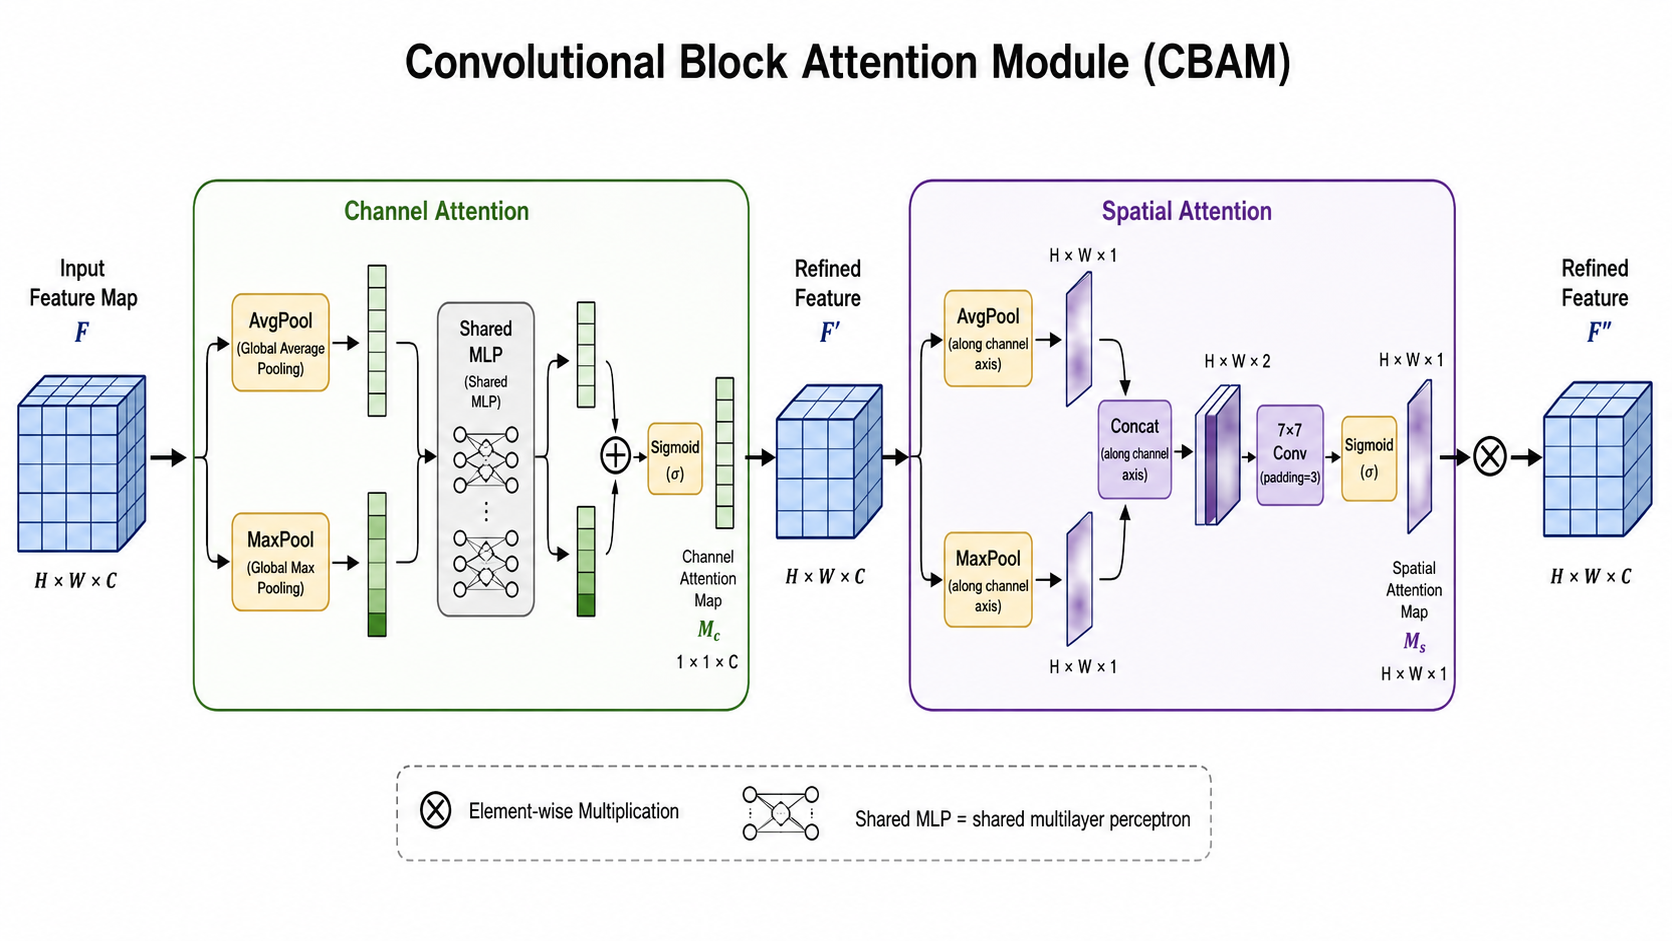
\includegraphics[width=0.90\textwidth]{figures/cbam_structure.png}
\caption{Structure of the Convolutional Block Attention Module. CBAM sequentially applies channel attention and spatial attention to refine the feature maps generated by the MobileNetV2 backbone.}
\label{fig:cbam_structure}
\end{figure}

\subsection{Integration of CBAM with MobileNetV2}

The late placement applies attention once to the most semantically developed convolutional map, avoiding repeated attention blocks throughout the backbone. It is a low-intervention design choice rather than a demonstrated optimum. The comparison with unmodified MobileNetV2 establishes its incremental cost, whereas early-, middle-, and post-pooling placements require a dedicated placement ablation.

In the proposed framework, CBAM is integrated after the final convolutional feature maps generated by the MobileNetV2 backbone and before the classification head. This integration strategy allows MobileNetV2 to first extract compact feature representations using its lightweight convolutional structure, after which CBAM refines these features by emphasizing disease-relevant channels and spatial regions.

Let $F_m$ denote the feature maps produced by the MobileNetV2 backbone:

\begin{equation}
    F_m = F_{\text{MobileNetV2}}(X).
\end{equation}

The CBAM module then refines these feature maps:

\begin{equation}
    F_a = \text{CBAM}(F_m),
\end{equation}

where $F_a$ represents the attention-enhanced feature map. The refined feature representation is passed through global average pooling:

\begin{equation}
    z = \text{GAP}(F_a).
\end{equation}

Finally, the output vector is passed to a dense classification layer with softmax activation:

\begin{equation}
    \hat{y}_i = \frac{e^{z_i}}{\sum_{j=1}^{K} e^{z_j}},
\end{equation}

where $\hat{y}_i$ is the predicted probability for class $i$, and $K$ is the total number of plant disease classes. In this study, $K=38$.

This design improves the representational capacity of MobileNetV2 while maintaining a lightweight architecture. By adding attention after feature extraction rather than replacing the backbone with a substantially heavier model, the proposed framework aims to balance classification accuracy and computational efficiency.

\subsection{Classification Head}

The classification head receives the attention-enhanced feature representation and maps it to the final disease classes. After CBAM refinement, global average pooling is applied to reduce the spatial dimensions of the feature maps while retaining channel-wise information. A dense layer with softmax activation is then used to produce the final class probability distribution.

The classification objective is optimized using categorical cross-entropy loss, defined as:

\begin{equation}
    \mathcal{L} = - \sum_{i=1}^{K} y_i \log(\hat{y}_i),
\end{equation}

where $y_i$ is the ground-truth label for class $i$, $\hat{y}_i$ is the predicted probability for class $i$, and $K$ is the number of classes. Since the dataset contains multiple plant disease categories, categorical cross-entropy is appropriate for the multi-class classification setting.

\subsection{Transfer Learning Strategy}

All models in this study were trained using transfer learning. The convolutional backbones were initialized with ImageNet pretrained weights, while the task-specific classification layers were trained on the PlantVillage dataset. Transfer learning was used to reduce training time and improve convergence by leveraging visual representations learned from large-scale image data.

For each backbone, all layers were first frozen and the final 30 layers were then unfrozen. The attention block and classification head were also trainable. This common partial-fine-tuning rule allowed deeper features to adapt to disease texture and morphology while limiting optimization cost. It also corrects the earlier description of the backbones as completely frozen. The present study does not compare different unfreezing depths; such an ablation remains necessary to establish whether 30 layers provide the best accuracy--cost trade-off.

\subsection{Proposed Model Summary}

The proposed MobileNetV2 + CBAM framework is designed to provide a balanced trade-off between classification performance and computational efficiency. MobileNetV2 contributes a compact and efficient feature extraction backbone, while CBAM enhances the extracted representations through channel and spatial attention. The model is therefore intended to improve the baseline lightweight architecture without introducing the high computational cost typically associated with deeper CNNs.

The key stages of the proposed method are summarized as follows:

\begin{enumerate}
    \item Input leaf images are resized to $224 \times 224$ pixels.
    \item Data augmentation is applied during training using rotation, zoom, horizontal flipping, and shear transformation.
    \item MobileNetV2 pretrained on ImageNet extracts lightweight convolutional feature maps.
    \item CBAM refines the extracted feature maps using sequential channel and spatial attention.
    \item Global average pooling converts the refined feature maps into a compact feature vector.
    \item A softmax classification layer predicts one of the 38 plant disease classes.
\end{enumerate}

\begin{table}[H]
\caption{Summary of the proposed MobileNetV2 + CBAM architecture.}
\label{tab:proposed_model_summary}
\centering
\begin{tabularx}{\textwidth}{p{3.0cm} p{4.0cm} X}
\toprule
\textbf{Stage} & \textbf{Component} & \textbf{Description} \\
\midrule
Input & Leaf image & Resized to $224 \times 224 \times 3$. \\
\addlinespace
Feature extraction & MobileNetV2 backbone & ImageNet-pretrained lightweight CNN with the final 30 layers unfrozen. \\
\addlinespace
Attention refinement & CBAM & Sequential channel and spatial attention applied to the final MobileNetV2 feature maps. \\
\addlinespace
Feature aggregation & Global Average Pooling & Converts the refined feature maps into a compact feature vector. \\
\addlinespace
Classification & Dense + Softmax & Predicts one of 38 healthy or diseased plant leaf classes. \\
\bottomrule
\end{tabularx}
\end{table}


%%%%%%%%%%%%%%%%%%%%%%%%%%%%%%%%%%%%%%%%%%
\section{Experimental Results}

\subsection{Experimental Setup}

Dataset partitioning, resizing, and augmentation are consolidated in Section~3.1. The held-out test set was used for the final classification results reported below.

Four transfer learning models were evaluated in this study: InceptionV3, MobileNetV2, MobileNetV2 + CBAM, and Xception. MobileNetV2 served as the lightweight baseline model, while MobileNetV2 + CBAM represented the proposed attention-enhanced architecture. InceptionV3 and Xception were included as comparative deep learning models to assess the trade-off between classification performance and computational efficiency.

All models were initialized with ImageNet weights. The final 30 backbone layers and the task-specific head were trainable; the earlier layers remained frozen. Training used at most 30 epochs, Adam with a learning rate of $1 \times 10^{-5}$, a batch size of 32, categorical cross-entropy, EarlyStopping, ReduceLROnPlateau, and ModelCheckpoint. The classification heads used global average pooling, dropout (0.4), a 1024-unit dense layer with $L_2=5\times10^{-4}$, a second dropout layer, and a 38-class softmax output.

Training was performed on a Windows 11 Pro laptop with an Intel Core i7-11800H CPU (8 cores/16 logical processors), 16 GB DDR4 RAM, and an NVIDIA GeForce RTX 3050 Ti Laptop GPU with 4 GB VRAM. The archived implementation used Python 3.10, TensorFlow 2.13, and Keras. Deployment reanalysis used TensorFlow Lite 2.18 with the XNNPACK CPU delegate on the same Intel processor. Latency was measured with eight CPU threads, batch size one, 50 warm-up invocations, and 200 timed invocations; image decoding and resizing were excluded. Median and 95th-percentile latency are reported because isolated means are sensitive to operating-system scheduling. These laptop-CPU measurements are reproducible platform-specific benchmarks, not smartphone or microcontroller measurements.

Accuracy was computed over all test samples. Precision, recall, and F1-score are weighted by class support; macro-averaged values are additionally discussed to reduce the influence of large classes. AUC is macro-averaged one-vs-rest across the 38 classes. Deployment indicators include parameter count, floating-point operations (FLOPs), approximate multiply--accumulate operations (MACs), serialized file size, dynamic-range-quantized TensorFlow Lite accuracy, and CPU latency.

\subsection{Results and Discussion}

Table~\ref{tab:model_comparison} reports a consistent re-evaluation of the saved H5 models using their trained input sizes and explicit averaging rules. Xception achieved the highest accuracy (98.30\%) and weighted F1-score (98.30\%). MobileNetV2 + CBAM achieved 97.17\% accuracy and 97.15\% weighted F1-score, compared with 96.78\% and 96.73\% for MobileNetV2. Thus, late CBAM increased accuracy by 0.39 percentage points in this re-evaluation. InceptionV3 achieved 96.89\% accuracy when evaluated at its trained $299\times299$ resolution; the substantially lower value in the earlier draft resulted from evaluating that model through a $224\times224$ comparison generator.

\begin{table}[H]
\caption{Re-evaluation of the saved floating-point models. Precision, recall, and F1 are support-weighted; AUC is macro one-vs-rest.}
\label{tab:model_comparison}
\centering
\small
\begin{tabularx}{\textwidth}{l c c c c c}
\toprule
\textbf{Model} & \textbf{Accuracy} & \textbf{Precision} & \textbf{Recall} & \textbf{F1-Score} & \textbf{AUC} \\
\midrule
InceptionV3~\cite{szegedy2016rethinking} & 96.89\% & 96.95\% & 96.89\% & 96.88\% & 99.96\% \\
MobileNetV2~\cite{sandler2018mobilenetv2} & 96.78\% & 96.93\% & 96.78\% & 96.73\% & 99.97\% \\
MobileNetV2 + CBAM~\cite{sandler2018mobilenetv2,woo2018cbam} & 97.17\% & 97.32\% & 97.17\% & 97.15\% & 99.97\% \\
Xception~\cite{chollet2017xception} & 98.30\% & 98.32\% & 98.30\% & 98.30\% & 99.98\% \\
\bottomrule
\end{tabularx}
\normalsize
\end{table}

To further analyze the learning behavior of the evaluated models, training and validation curves were examined. Figure~\ref{fig:training_validation_accuracy_loss} presents the accuracy and loss curves for InceptionV3, MobileNetV2, MobileNetV2 + CBAM, and Xception. These curves provide insight into convergence behavior and possible overfitting during training. Figure~\ref{fig:training_validation_auc} presents the corresponding training and validation AUC curves, which further illustrate the discriminative ability of the models across epochs.

\begin{figure}[H]
\centering
\subfloat[\centering InceptionV3]{
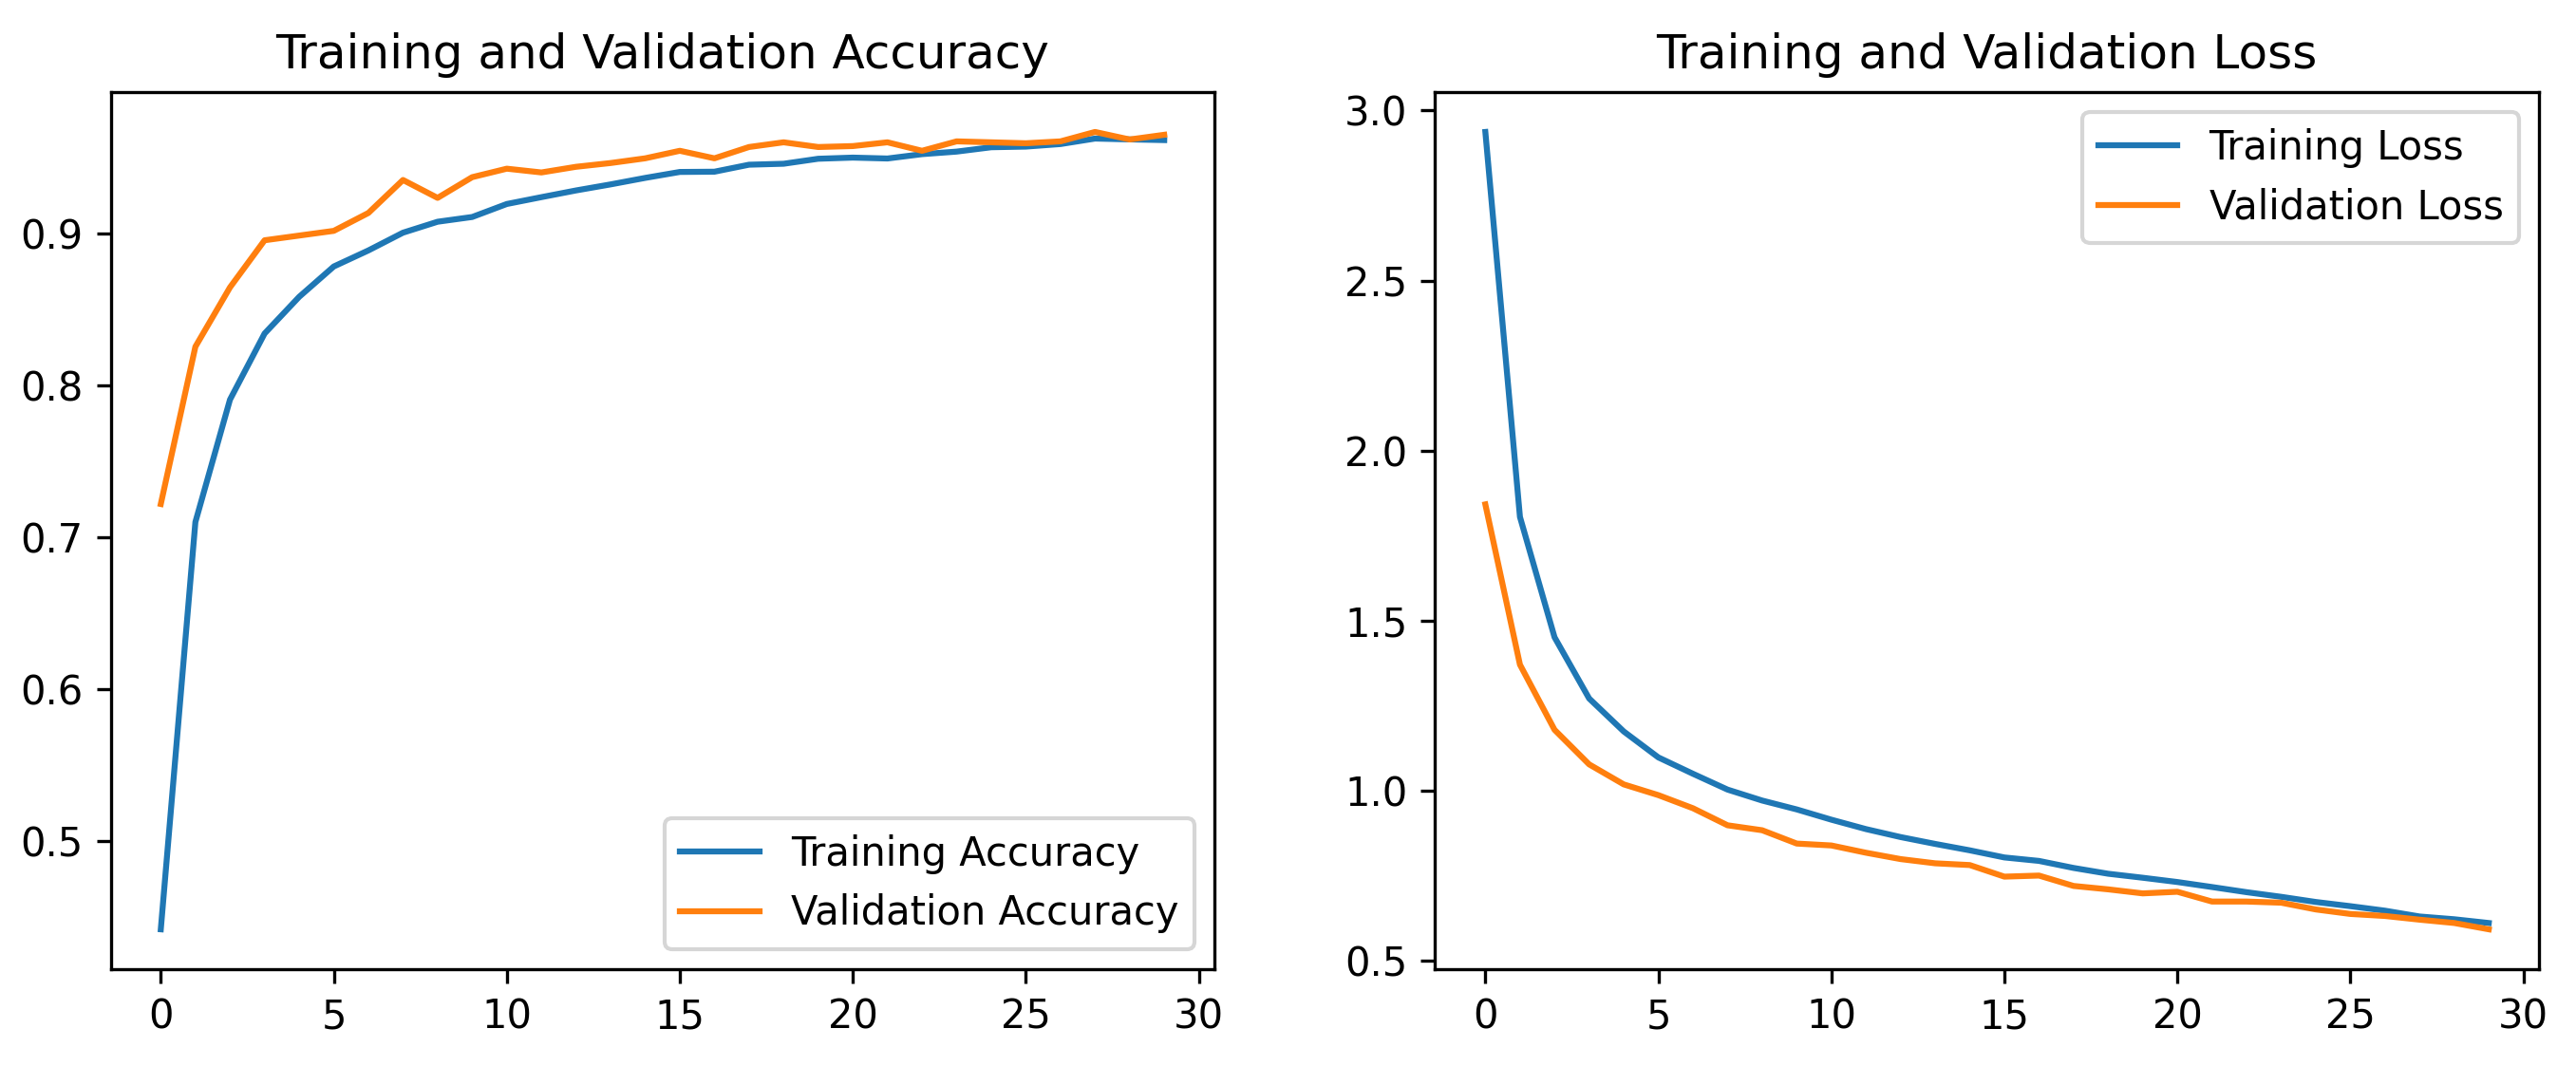
\includegraphics[width=0.47\textwidth]{figures/inceptionv3_accuracy_loss.png}
}
\hfill
\subfloat[\centering MobileNetV2]{
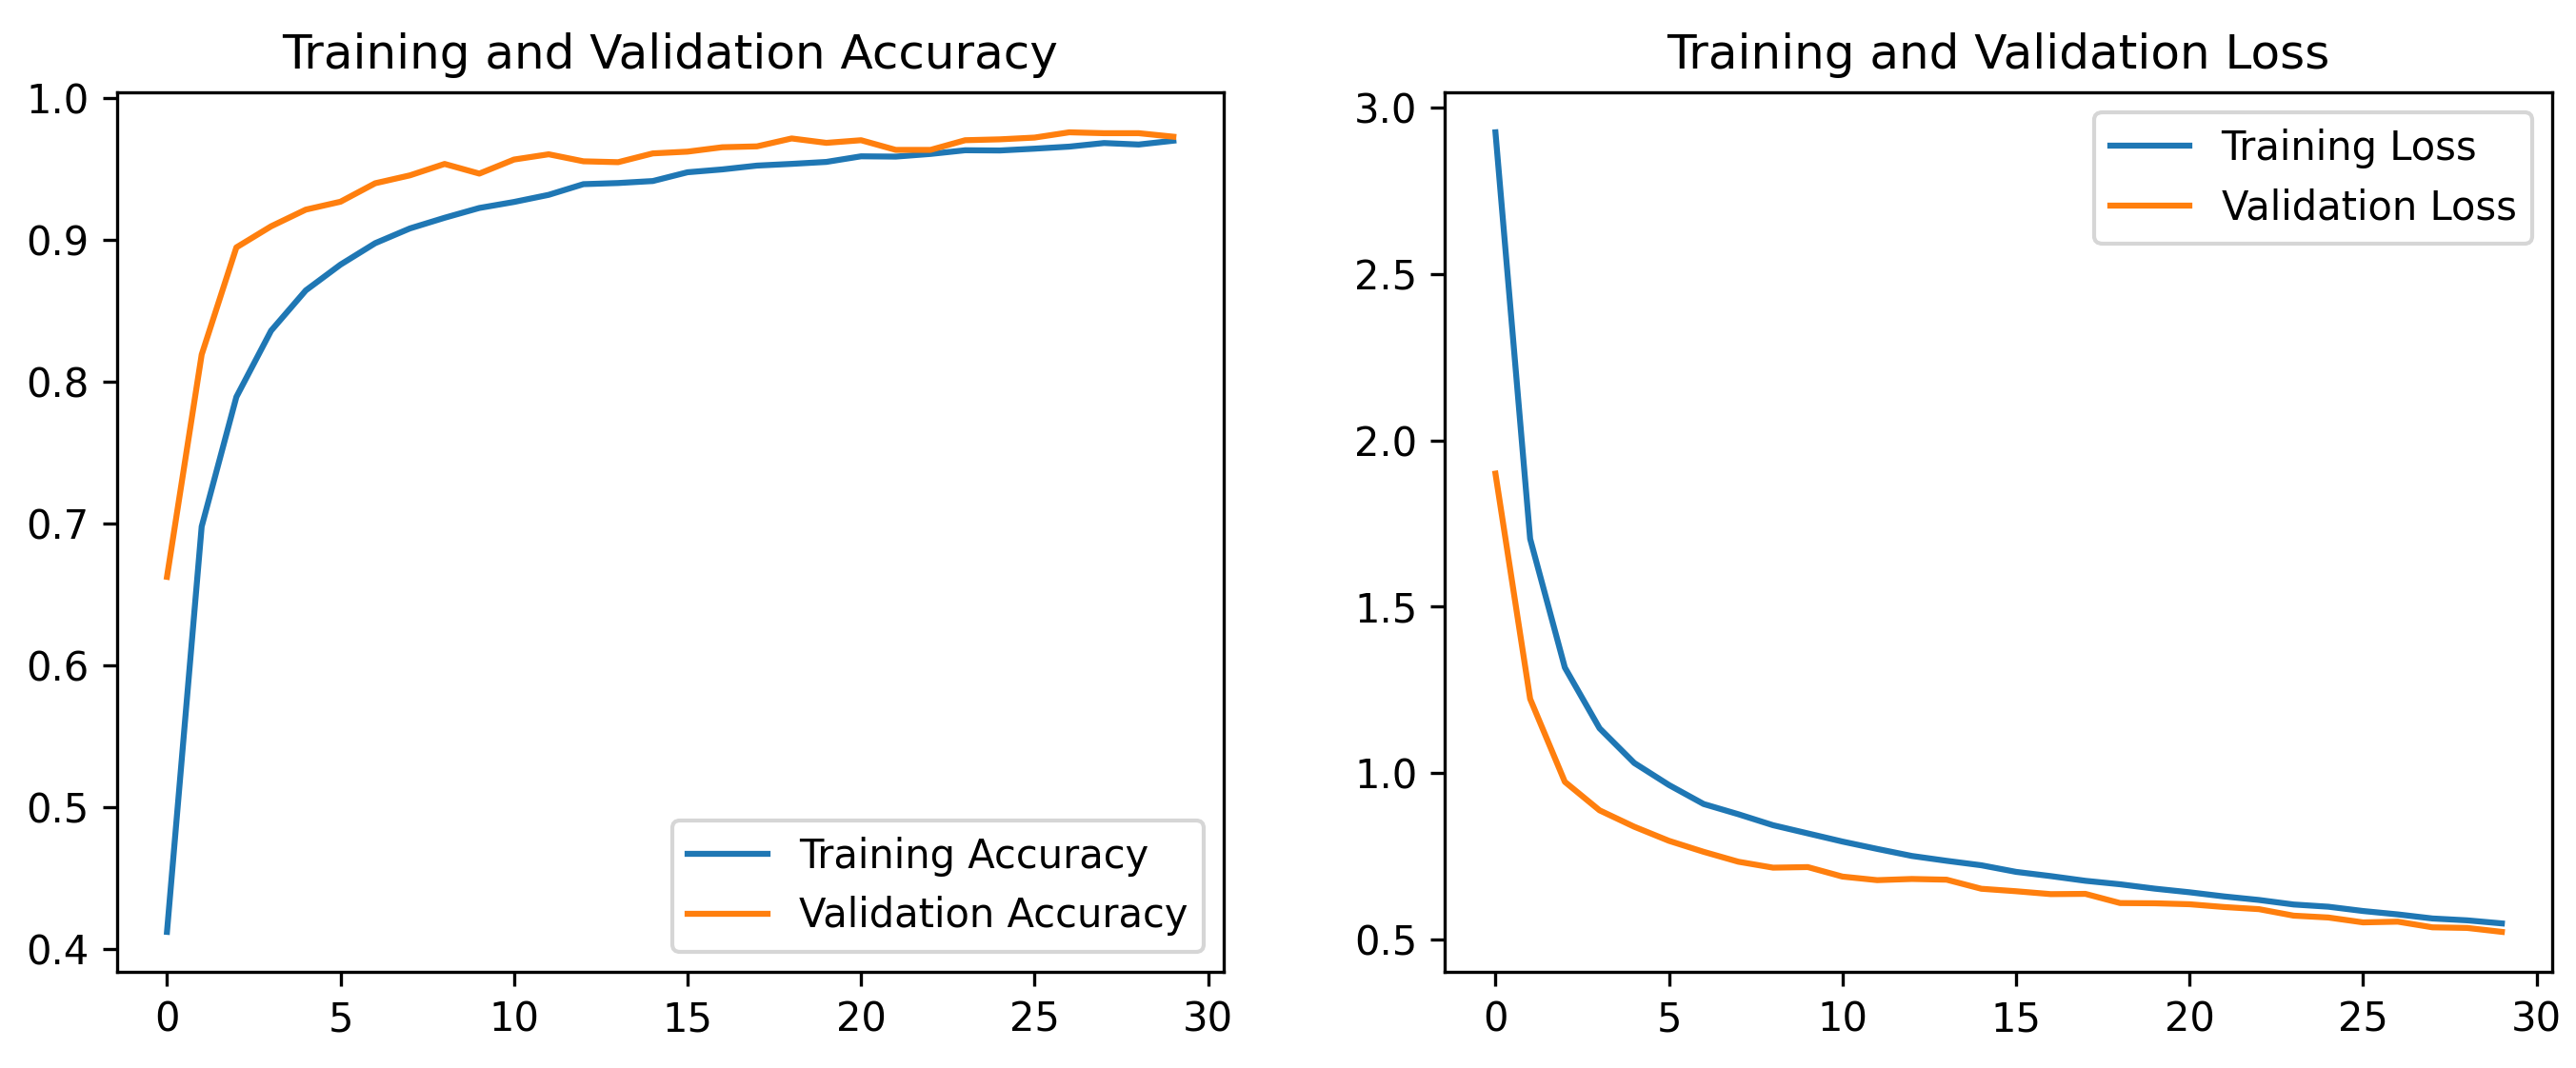
\includegraphics[width=0.47\textwidth]{figures/mobilenetv2_accuracy_loss.png}
}\\[3pt]
\subfloat[\centering MobileNetV2 + CBAM]{
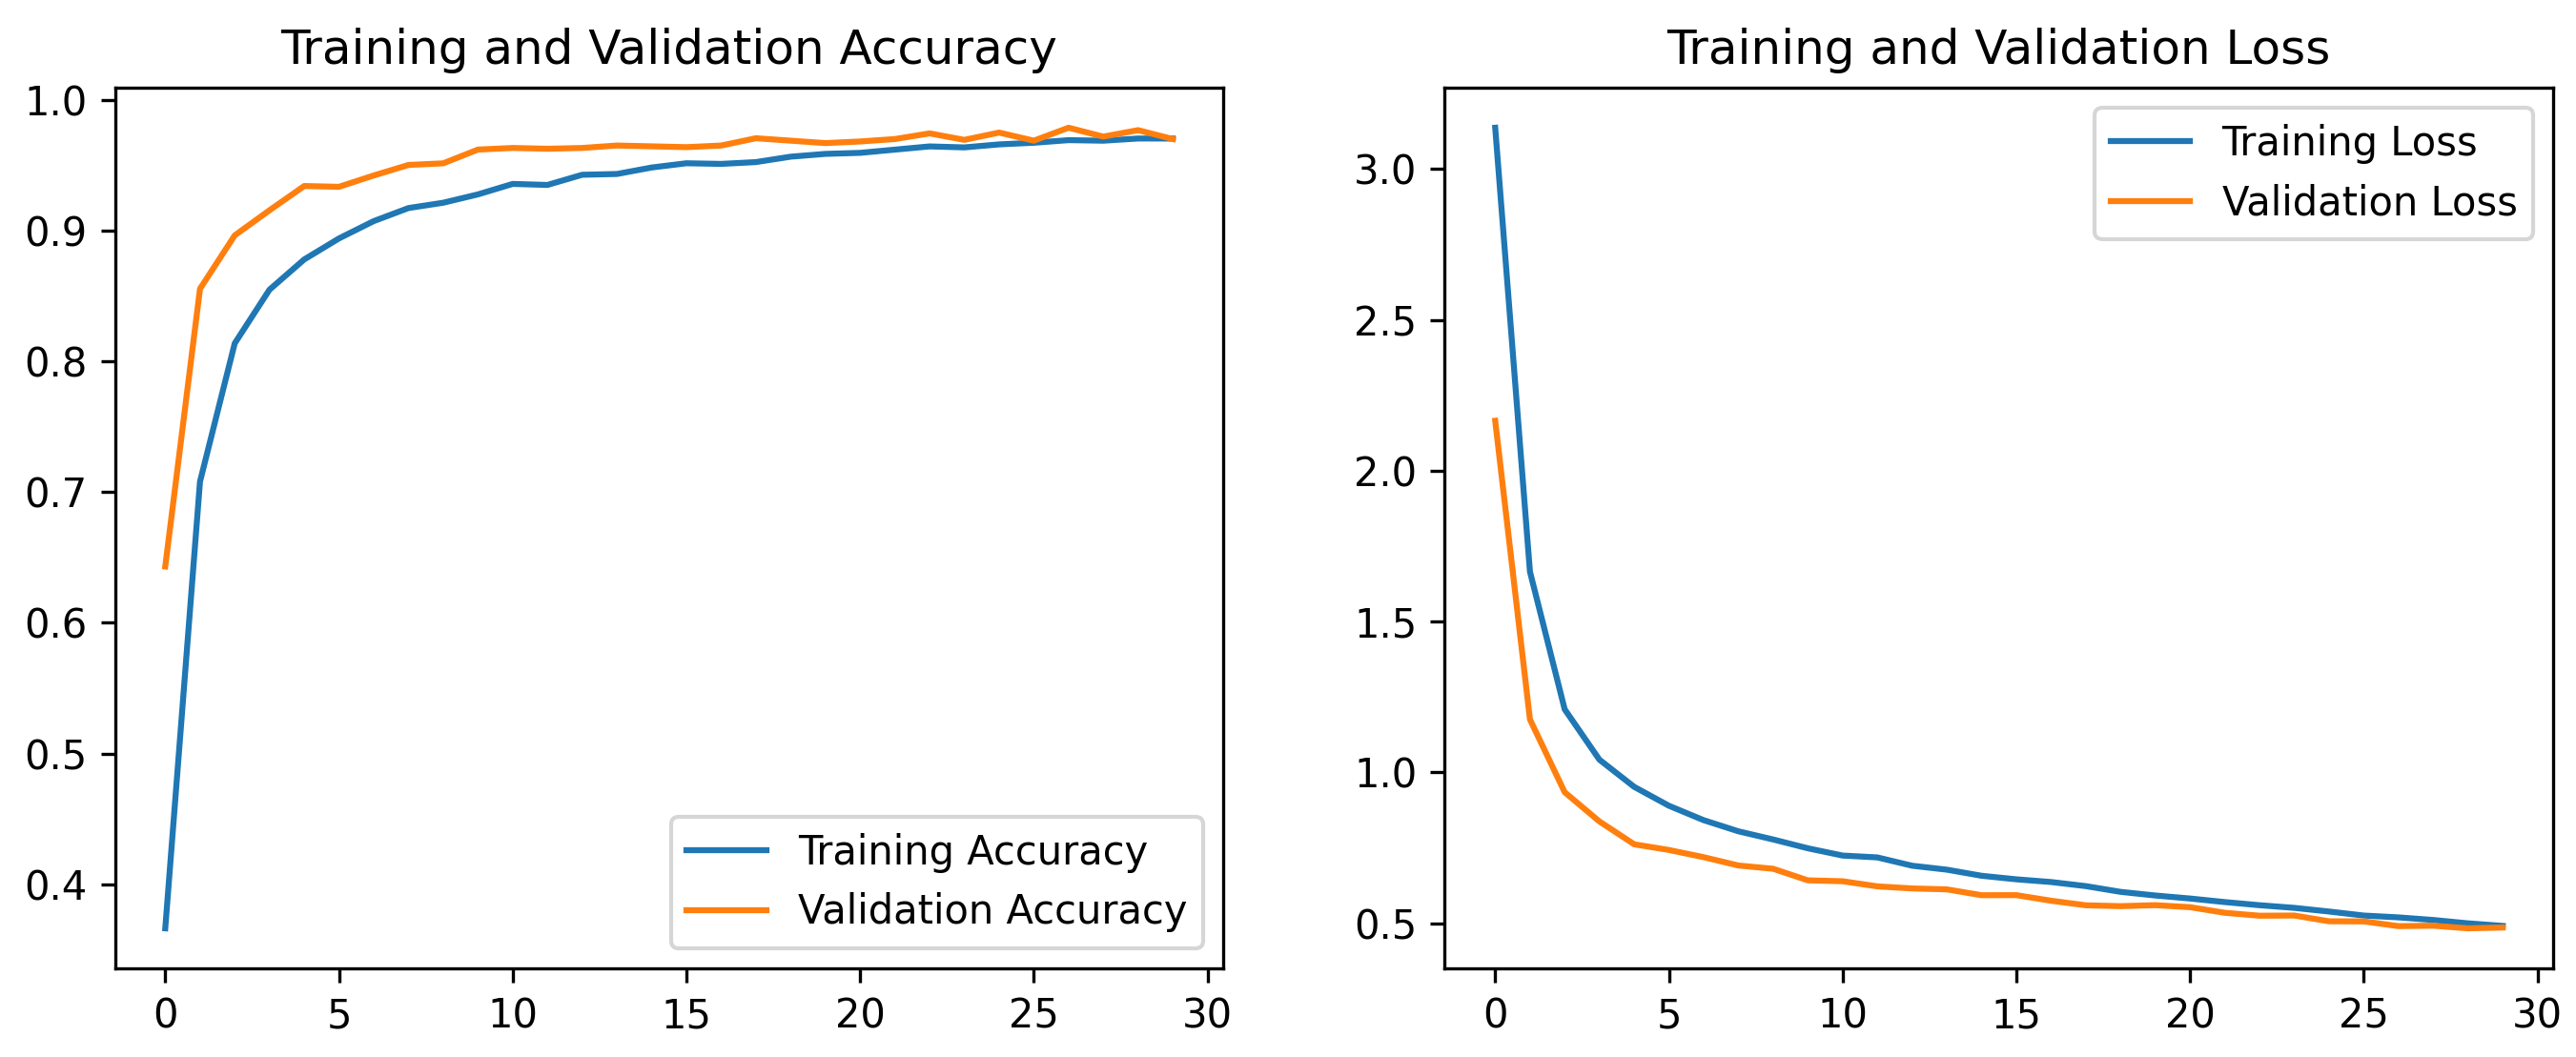
\includegraphics[width=0.47\textwidth]{figures/mobilenetv2_cbam_accuracy_loss.png}
}
\hfill
\subfloat[\centering Xception]{
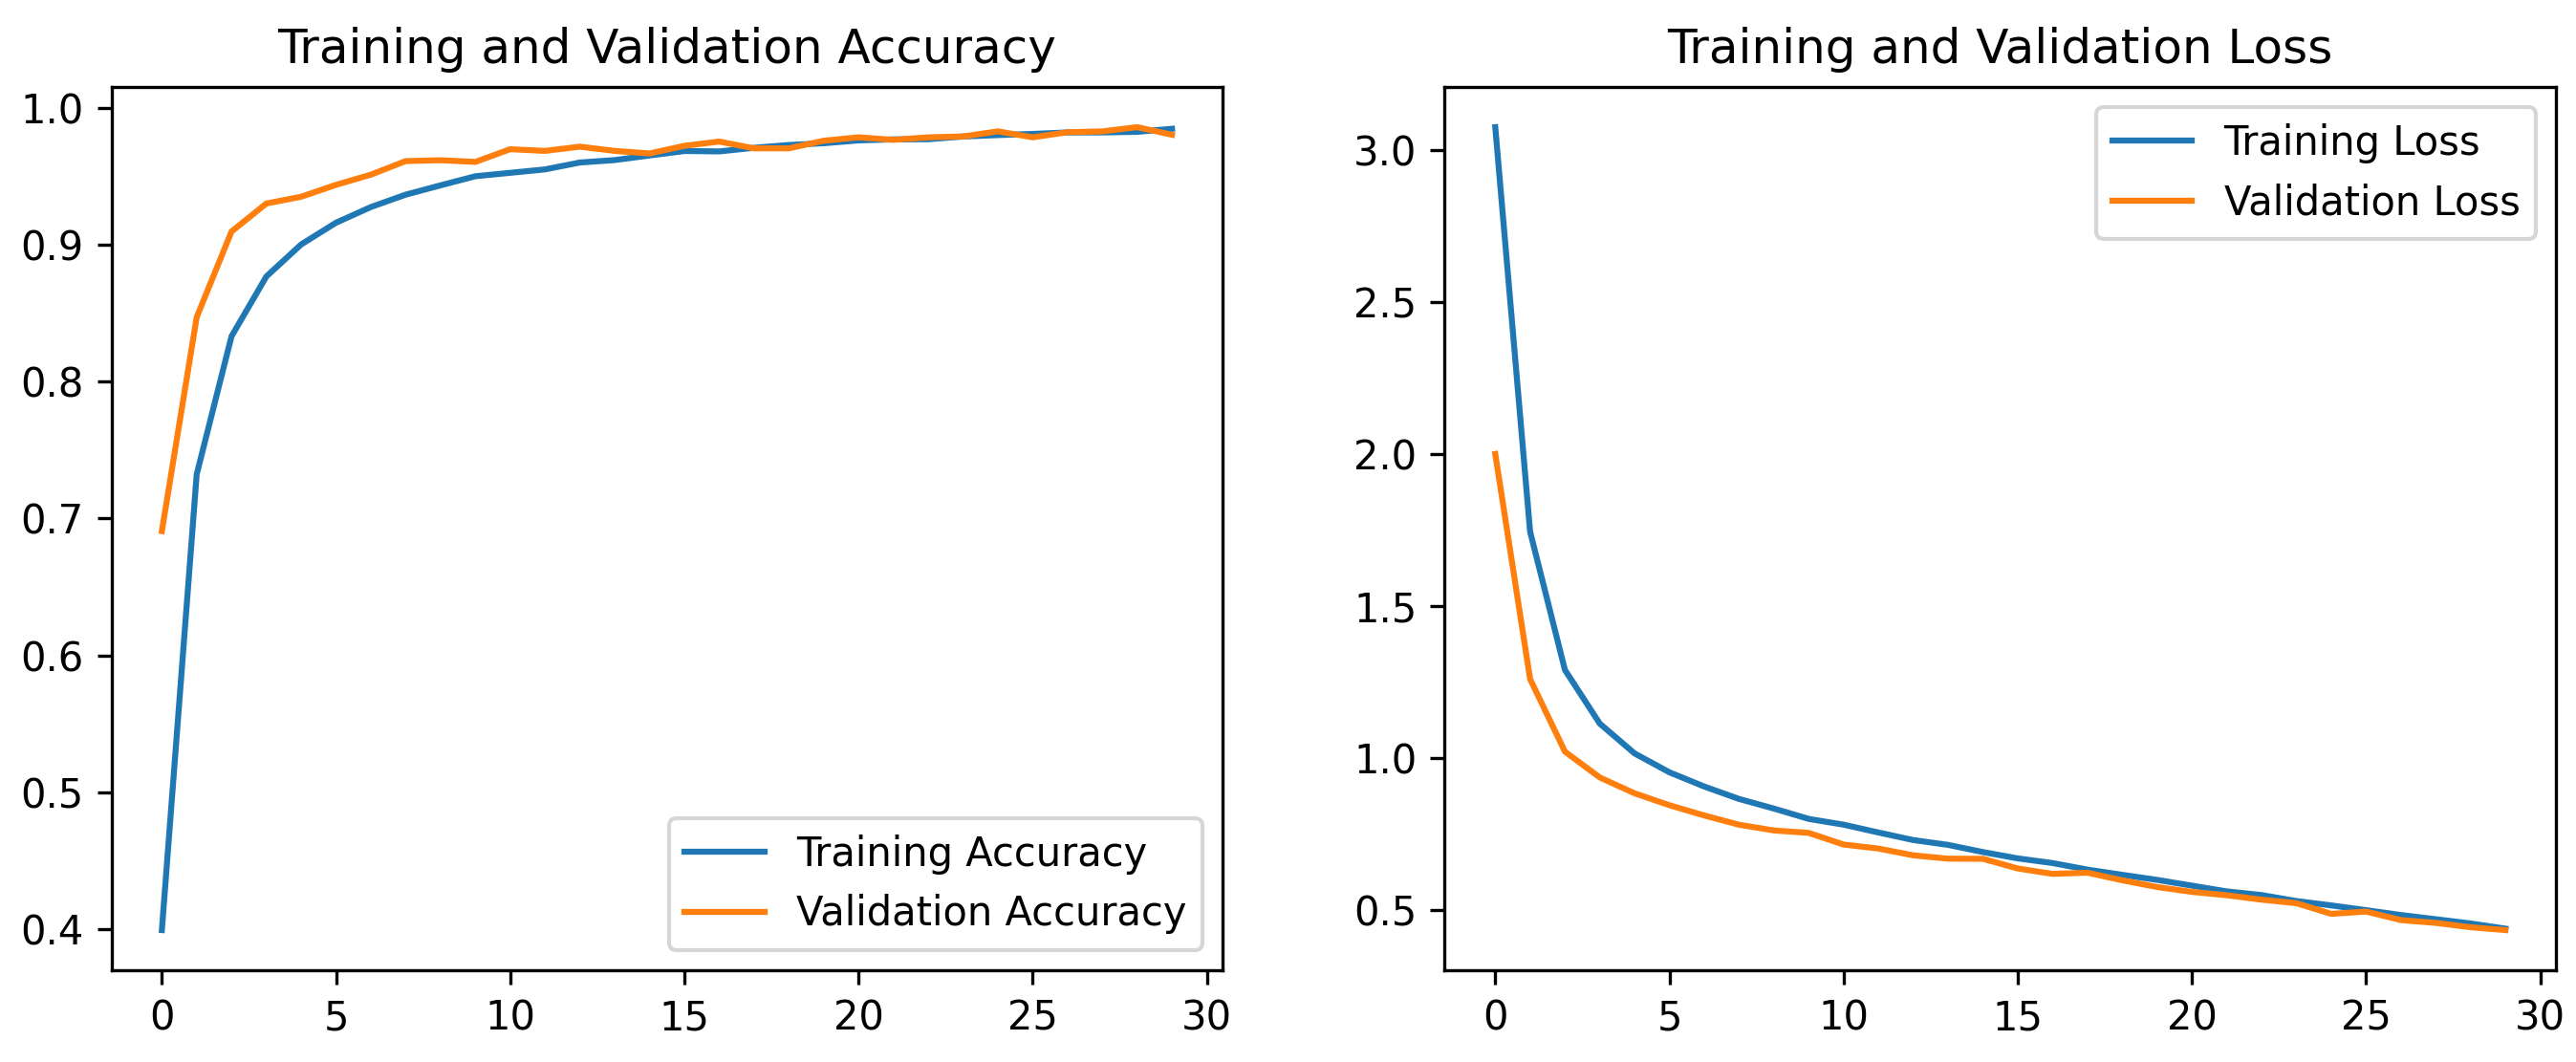
\includegraphics[width=0.47\textwidth]{figures/xception_accuracy_loss.png}
}
\caption{Training and validation accuracy/loss curves for the evaluated models. (\textbf{a}) InceptionV3. (\textbf{b}) MobileNetV2. (\textbf{c}) MobileNetV2 + CBAM. (\textbf{d}) Xception. The curves illustrate the learning behavior and convergence stability of each model during training.}
\label{fig:training_validation_accuracy_loss}
\end{figure}

\begin{figure}[H]
\centering
\subfloat[\centering InceptionV3]{
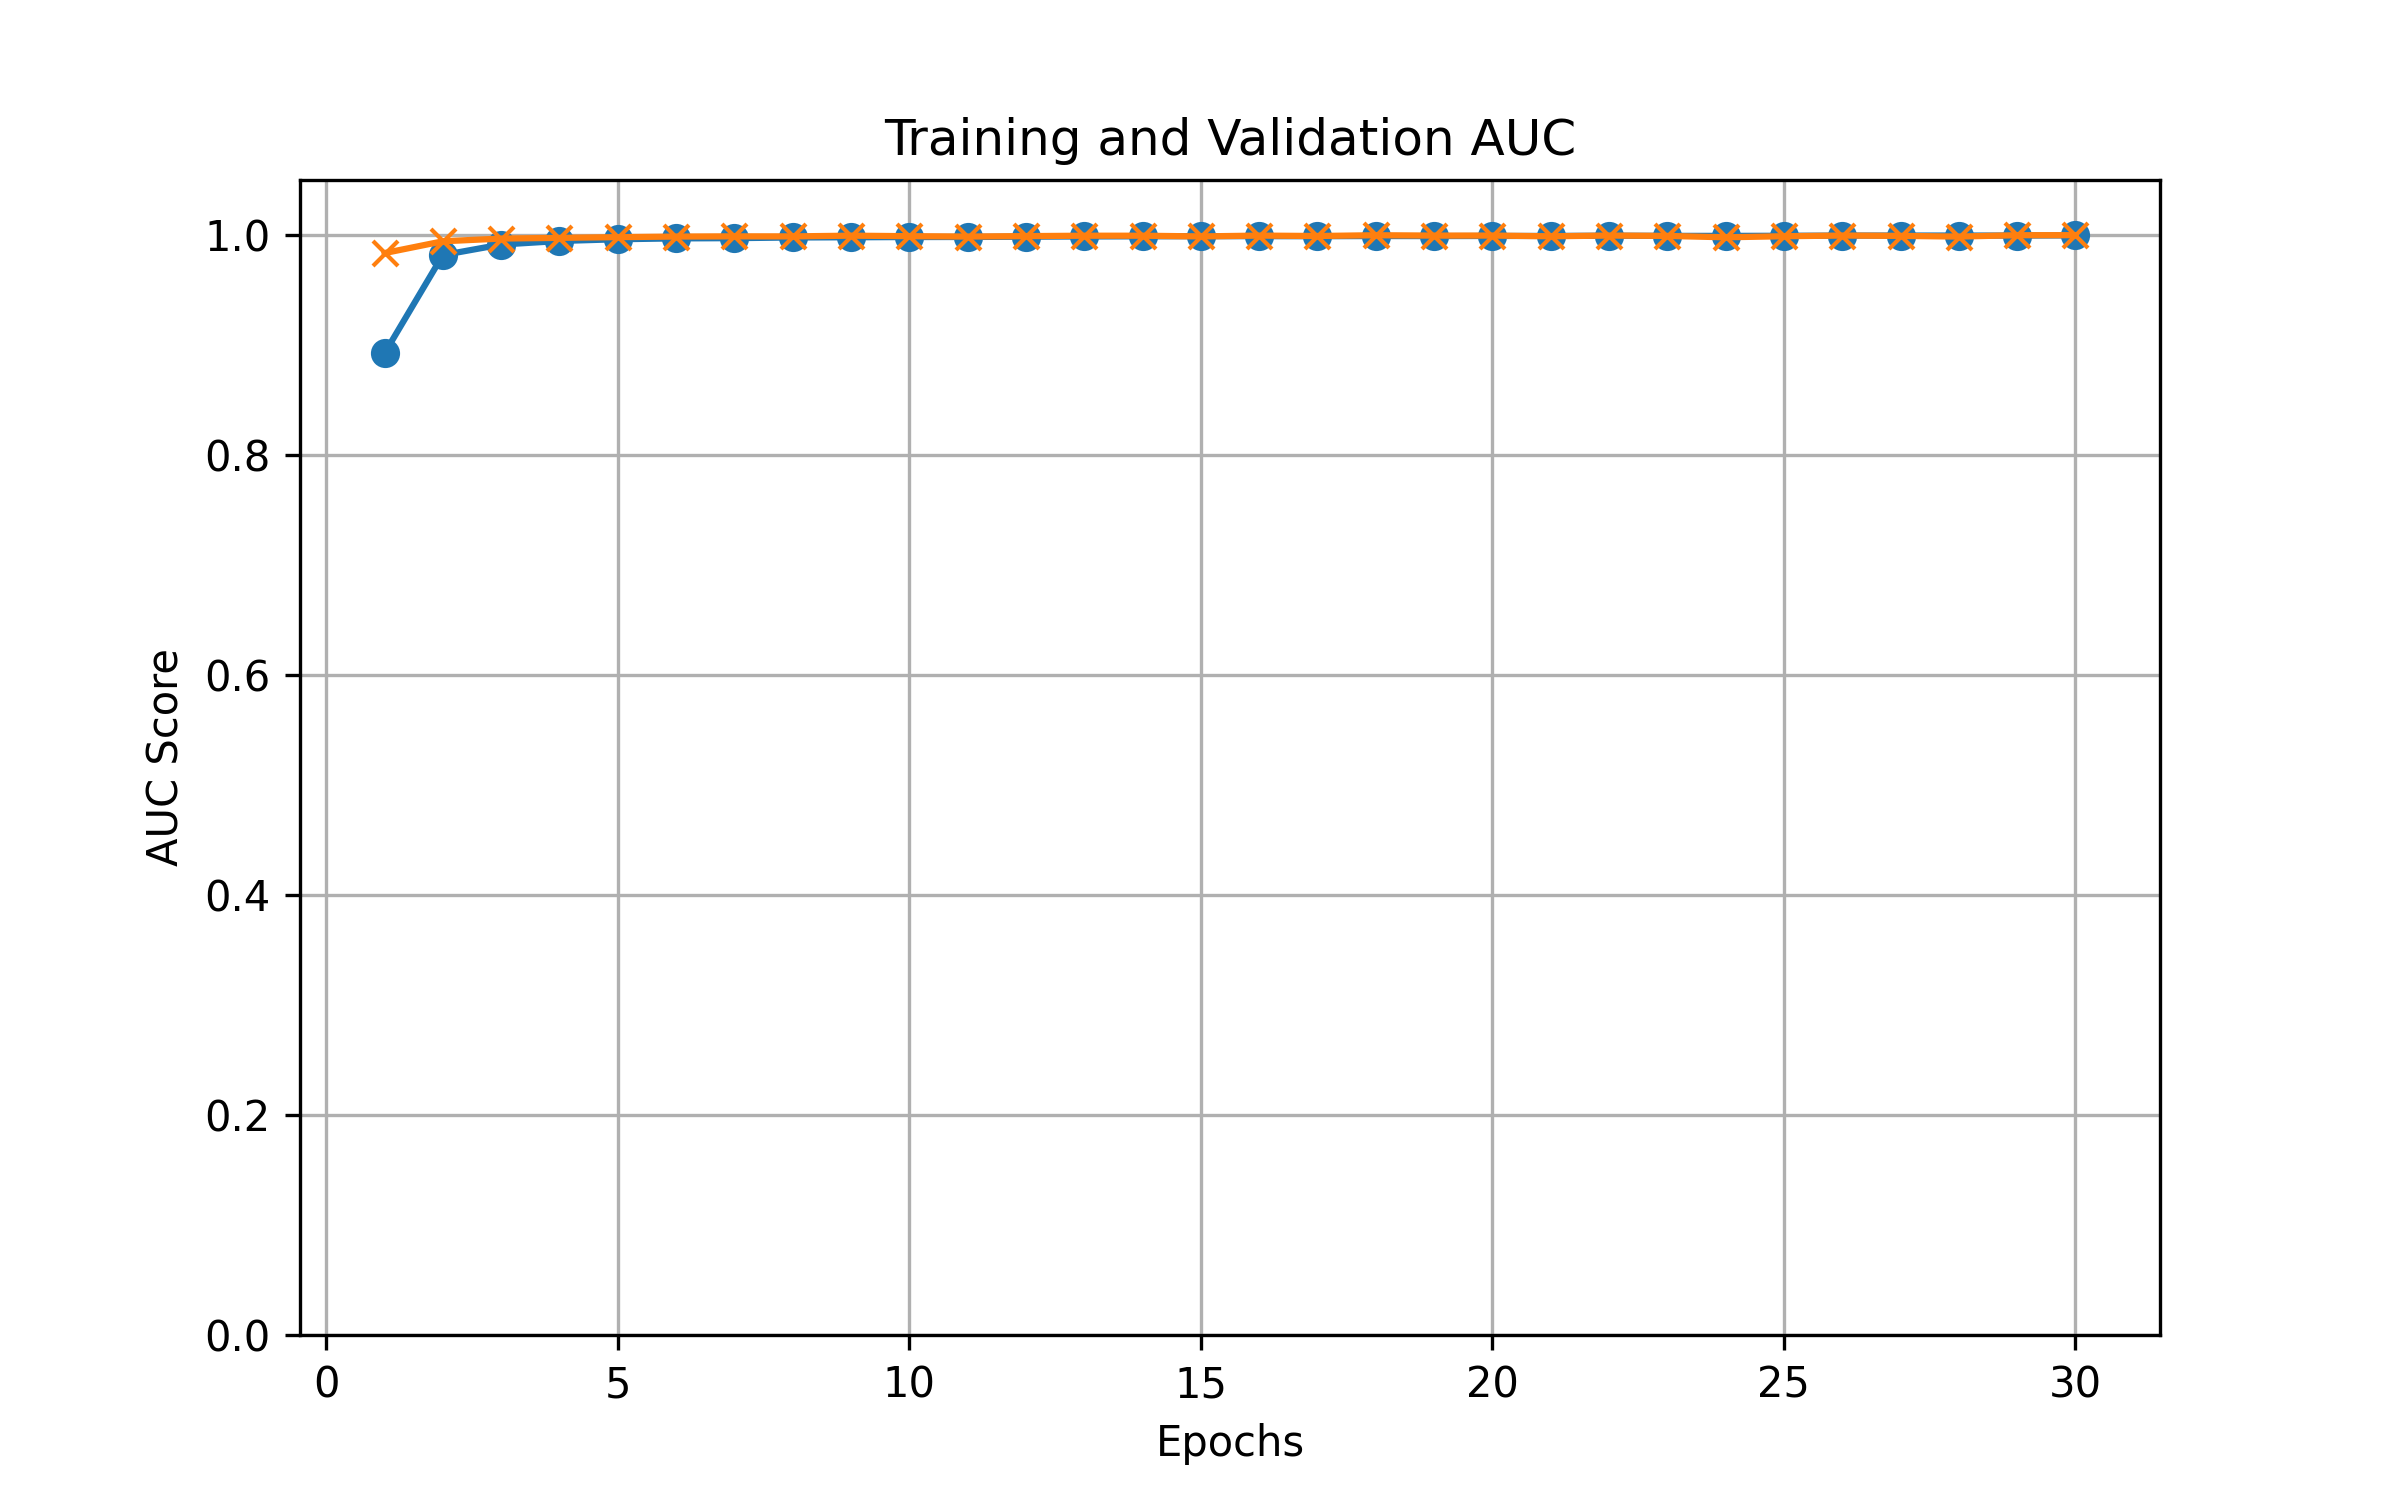
\includegraphics[width=0.47\textwidth]{figures/inceptionv3_auc.png}
}
\hfill
\subfloat[\centering MobileNetV2]{
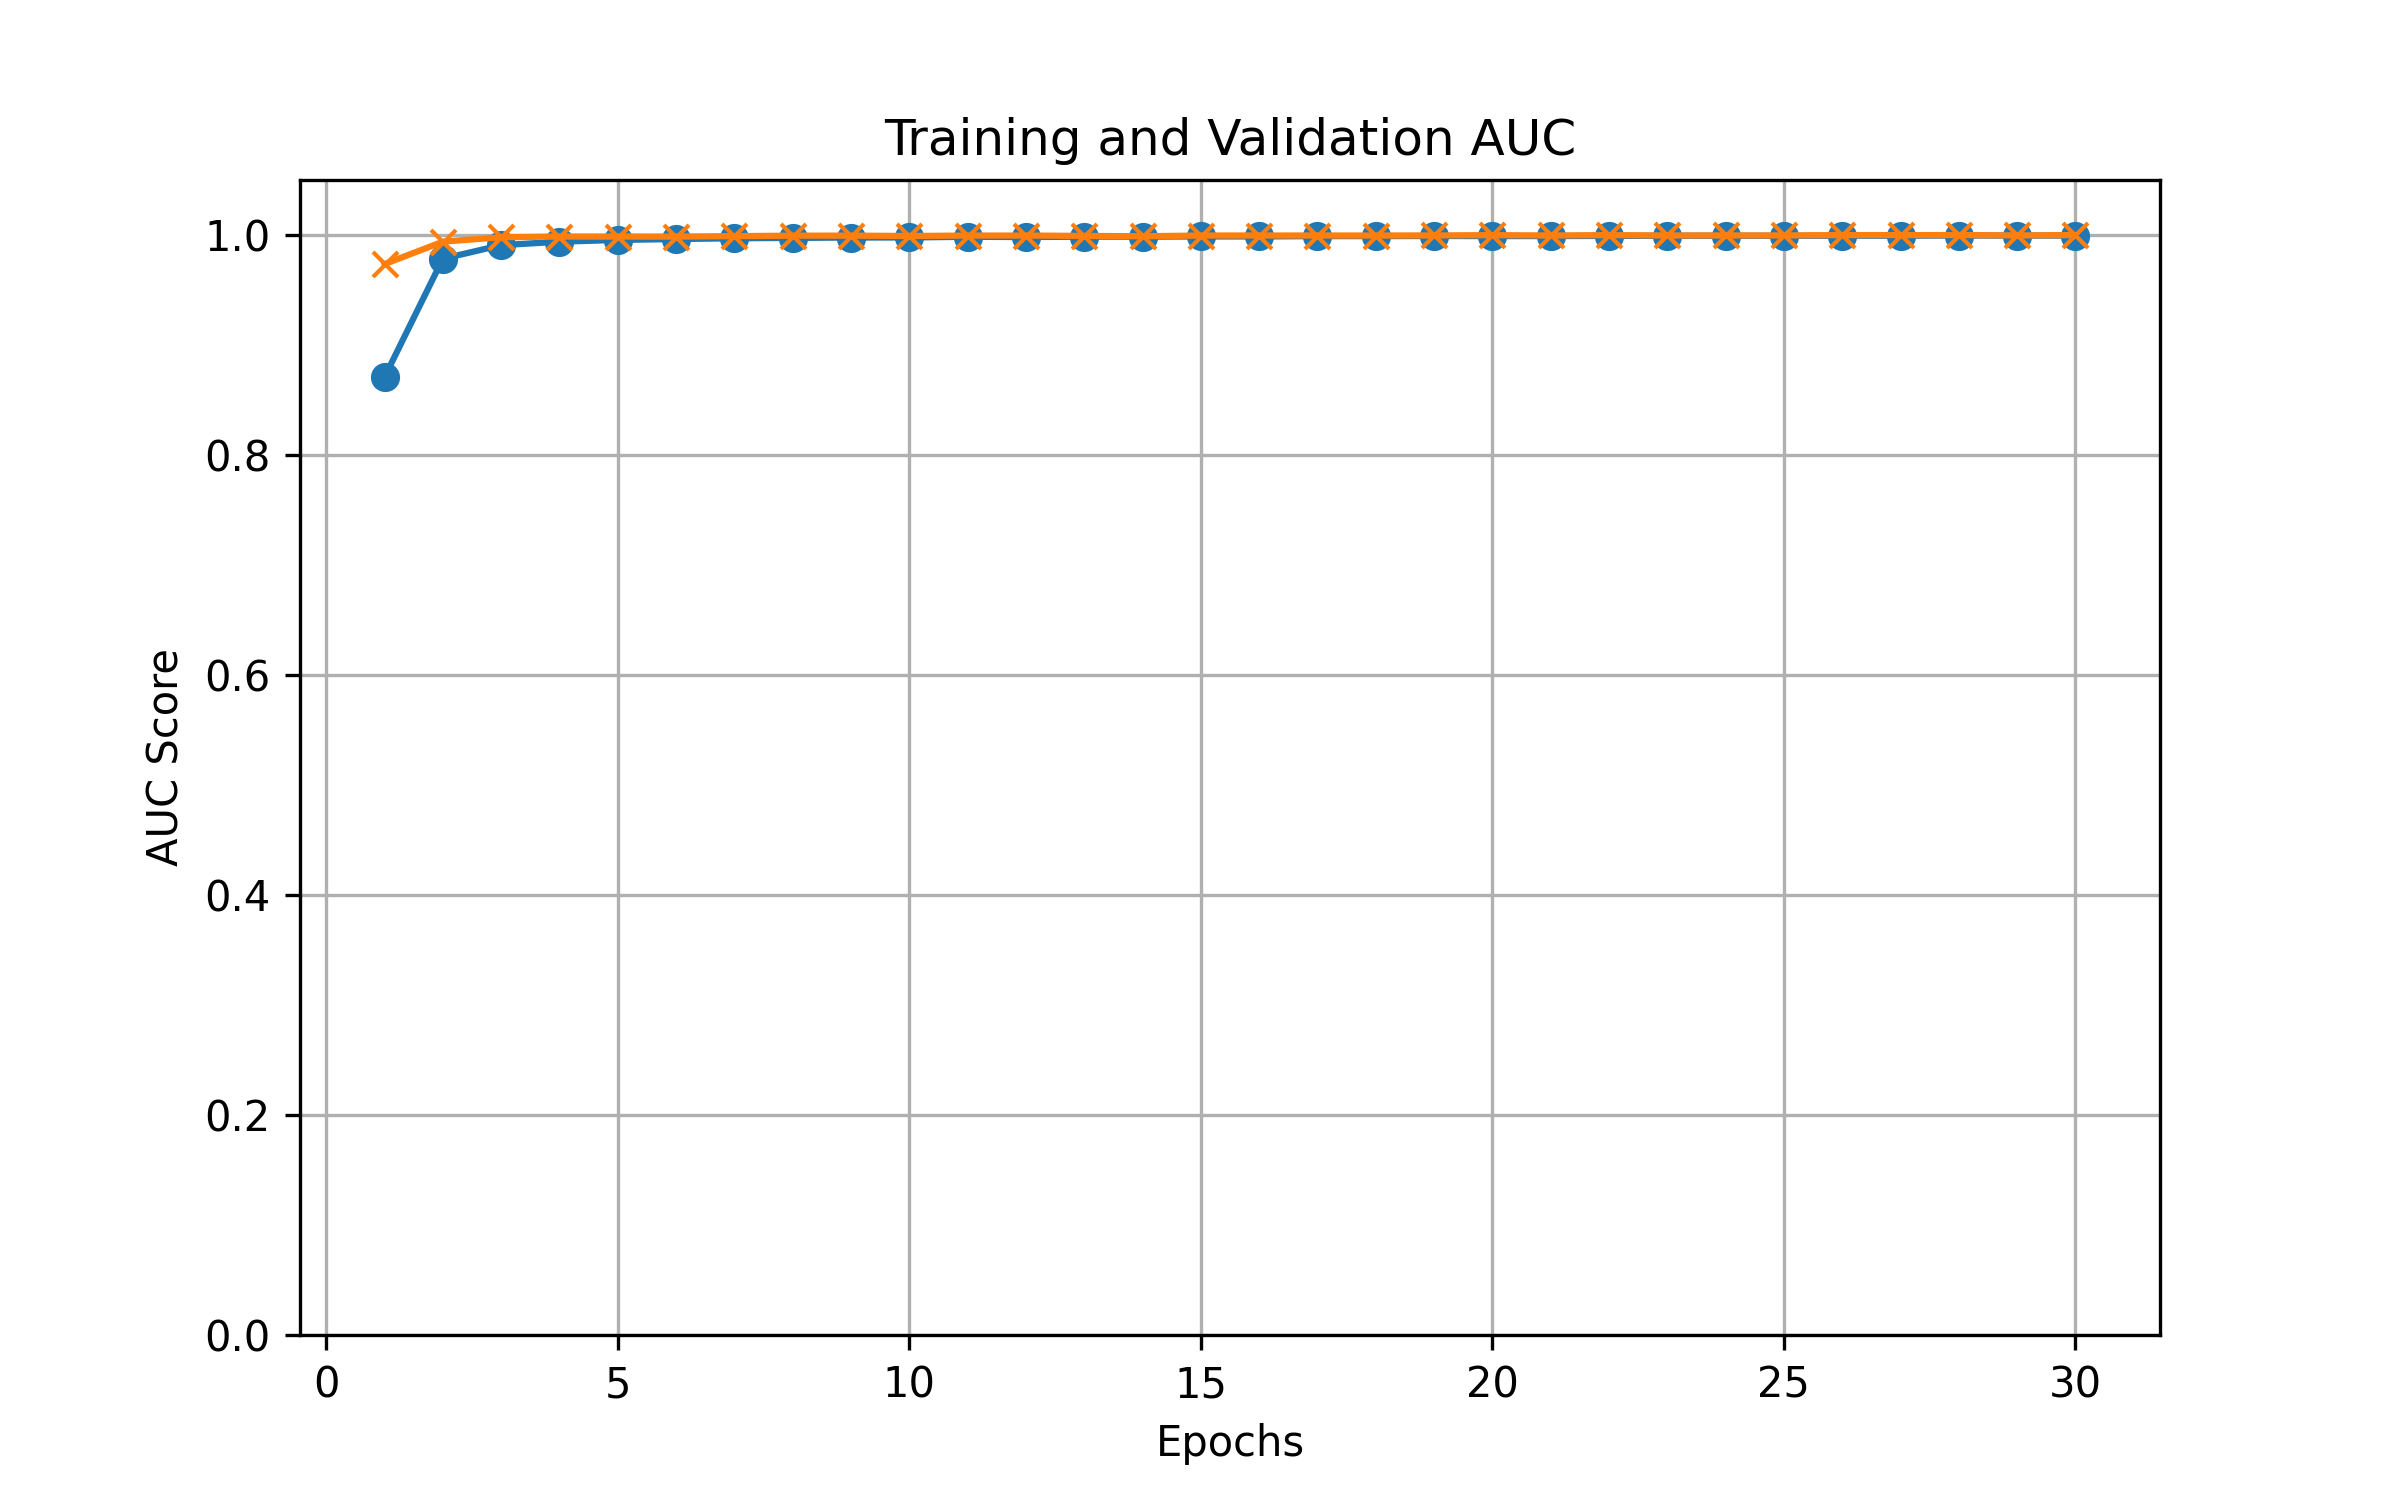
\includegraphics[width=0.47\textwidth]{figures/mobilenetv2_auc.png}
}\\[3pt]
\subfloat[\centering MobileNetV2 + CBAM]{
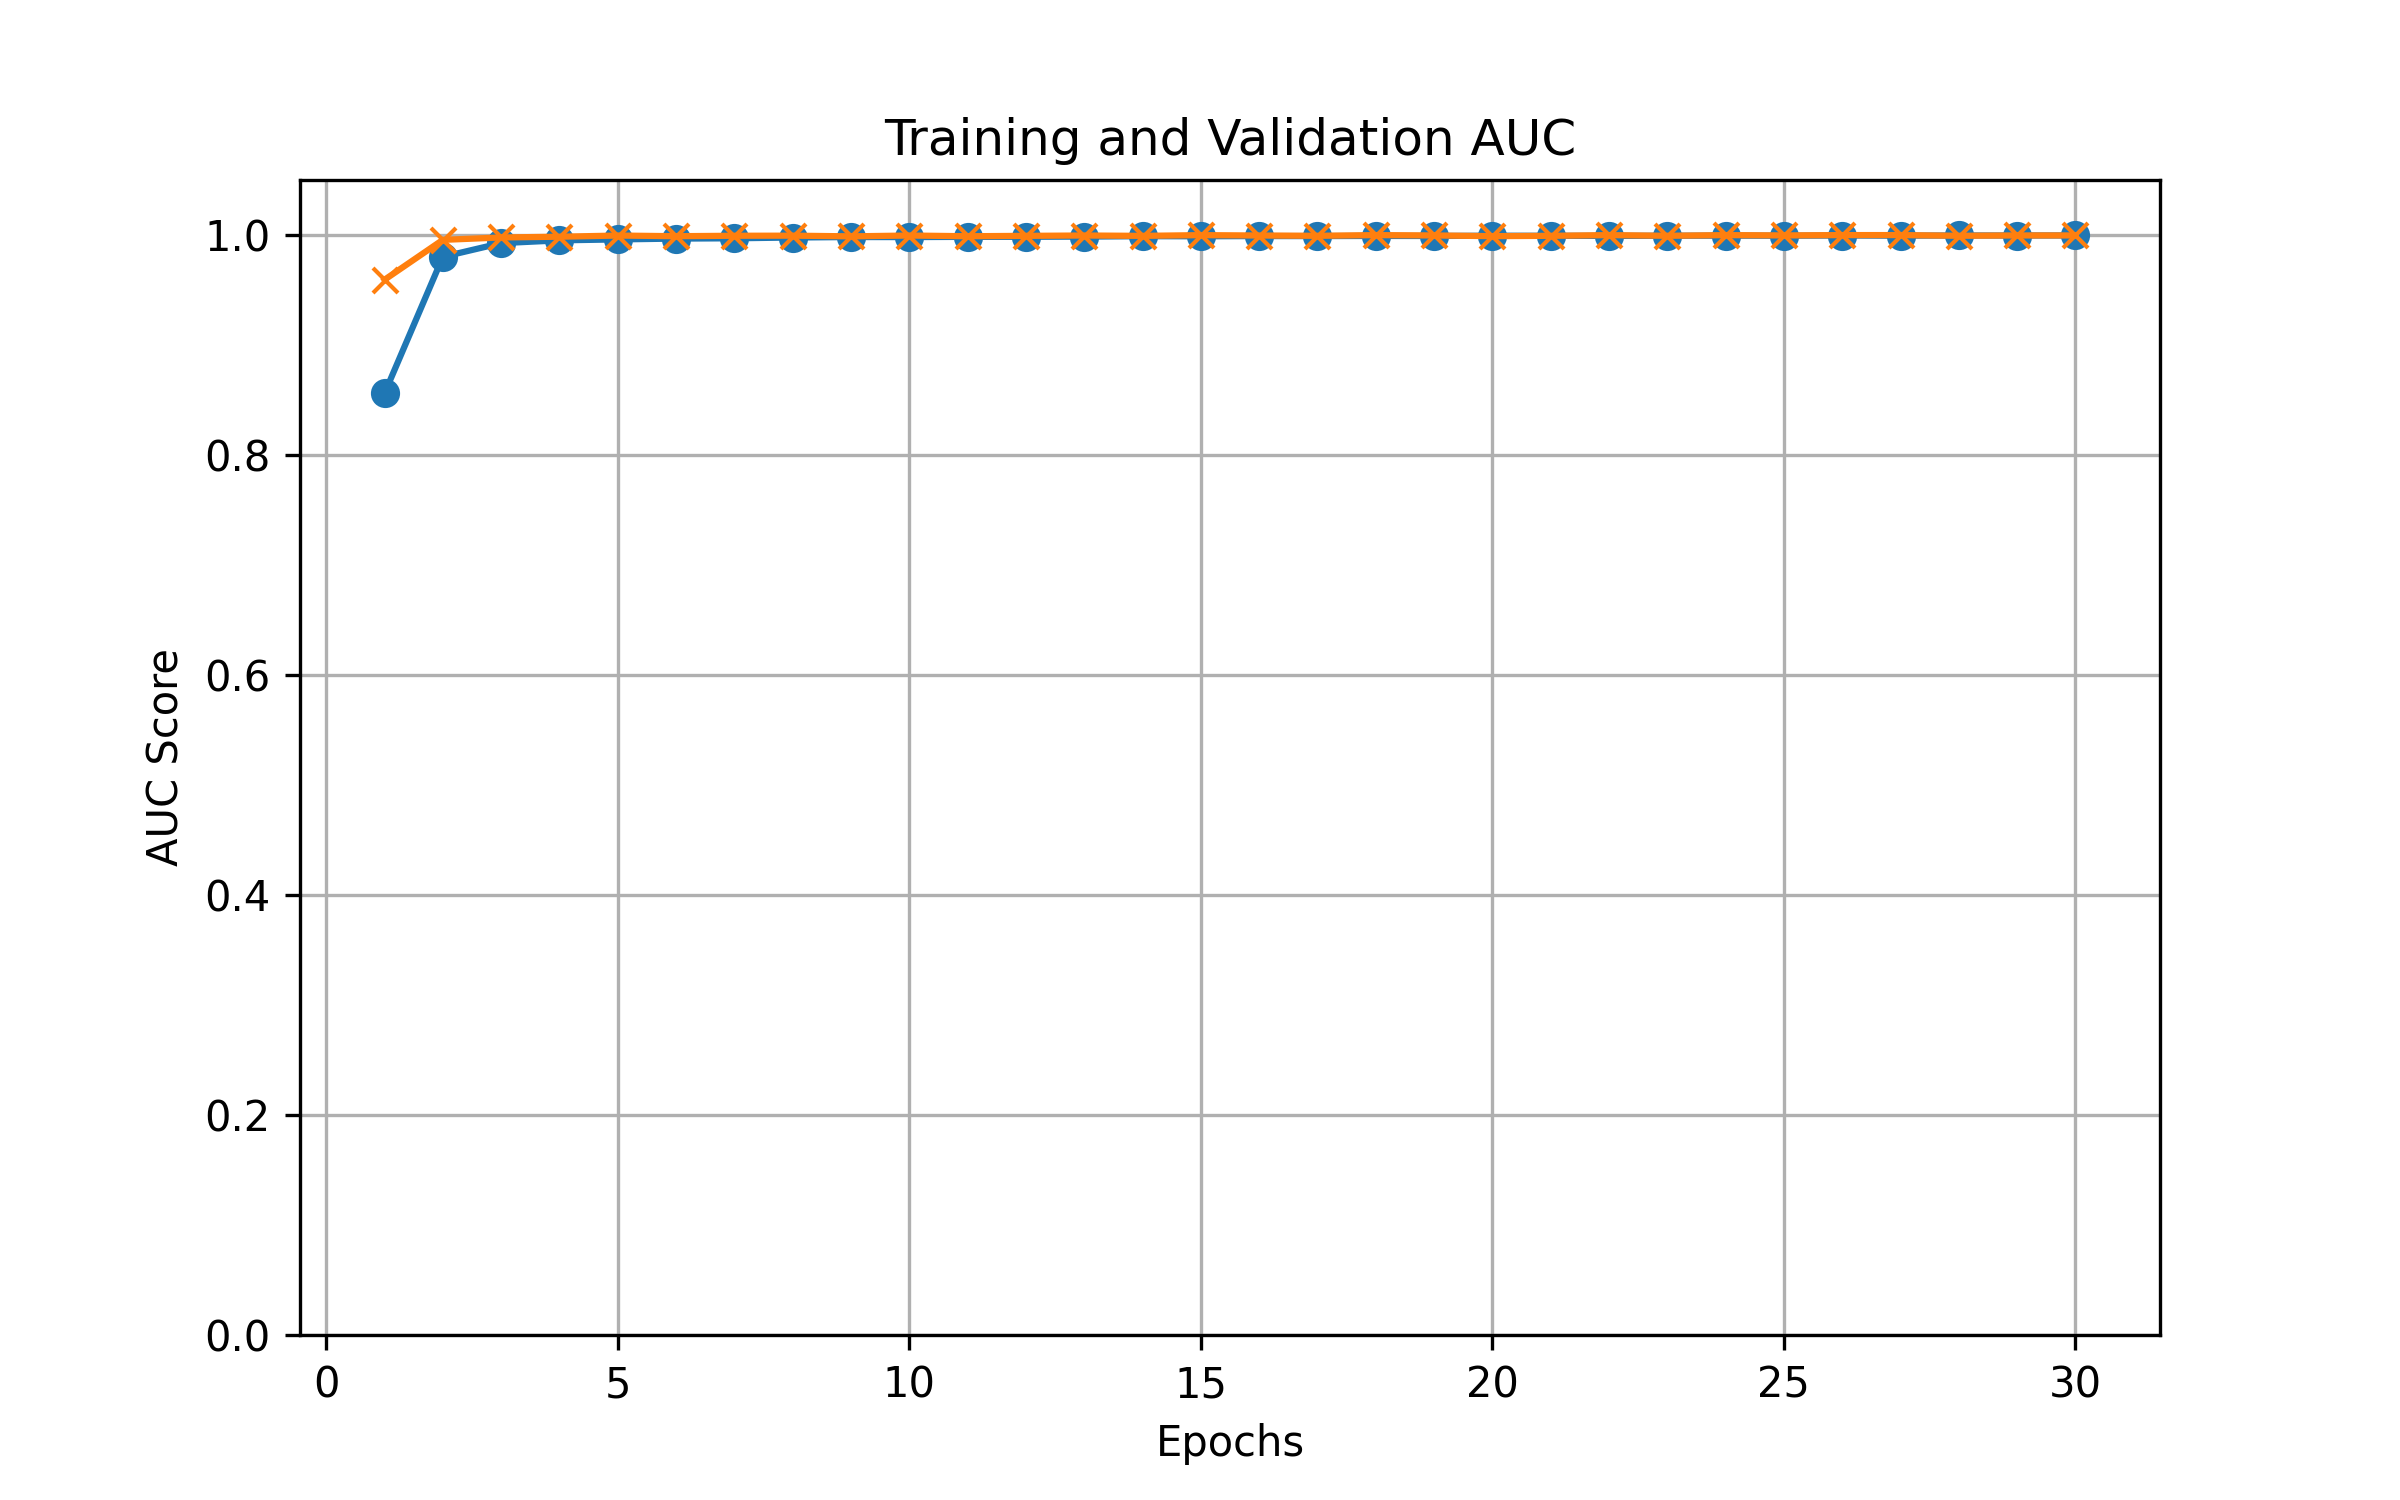
\includegraphics[width=0.47\textwidth]{figures/mobilenetv2_cbam_auc.png}
}
\hfill
\subfloat[\centering Xception]{
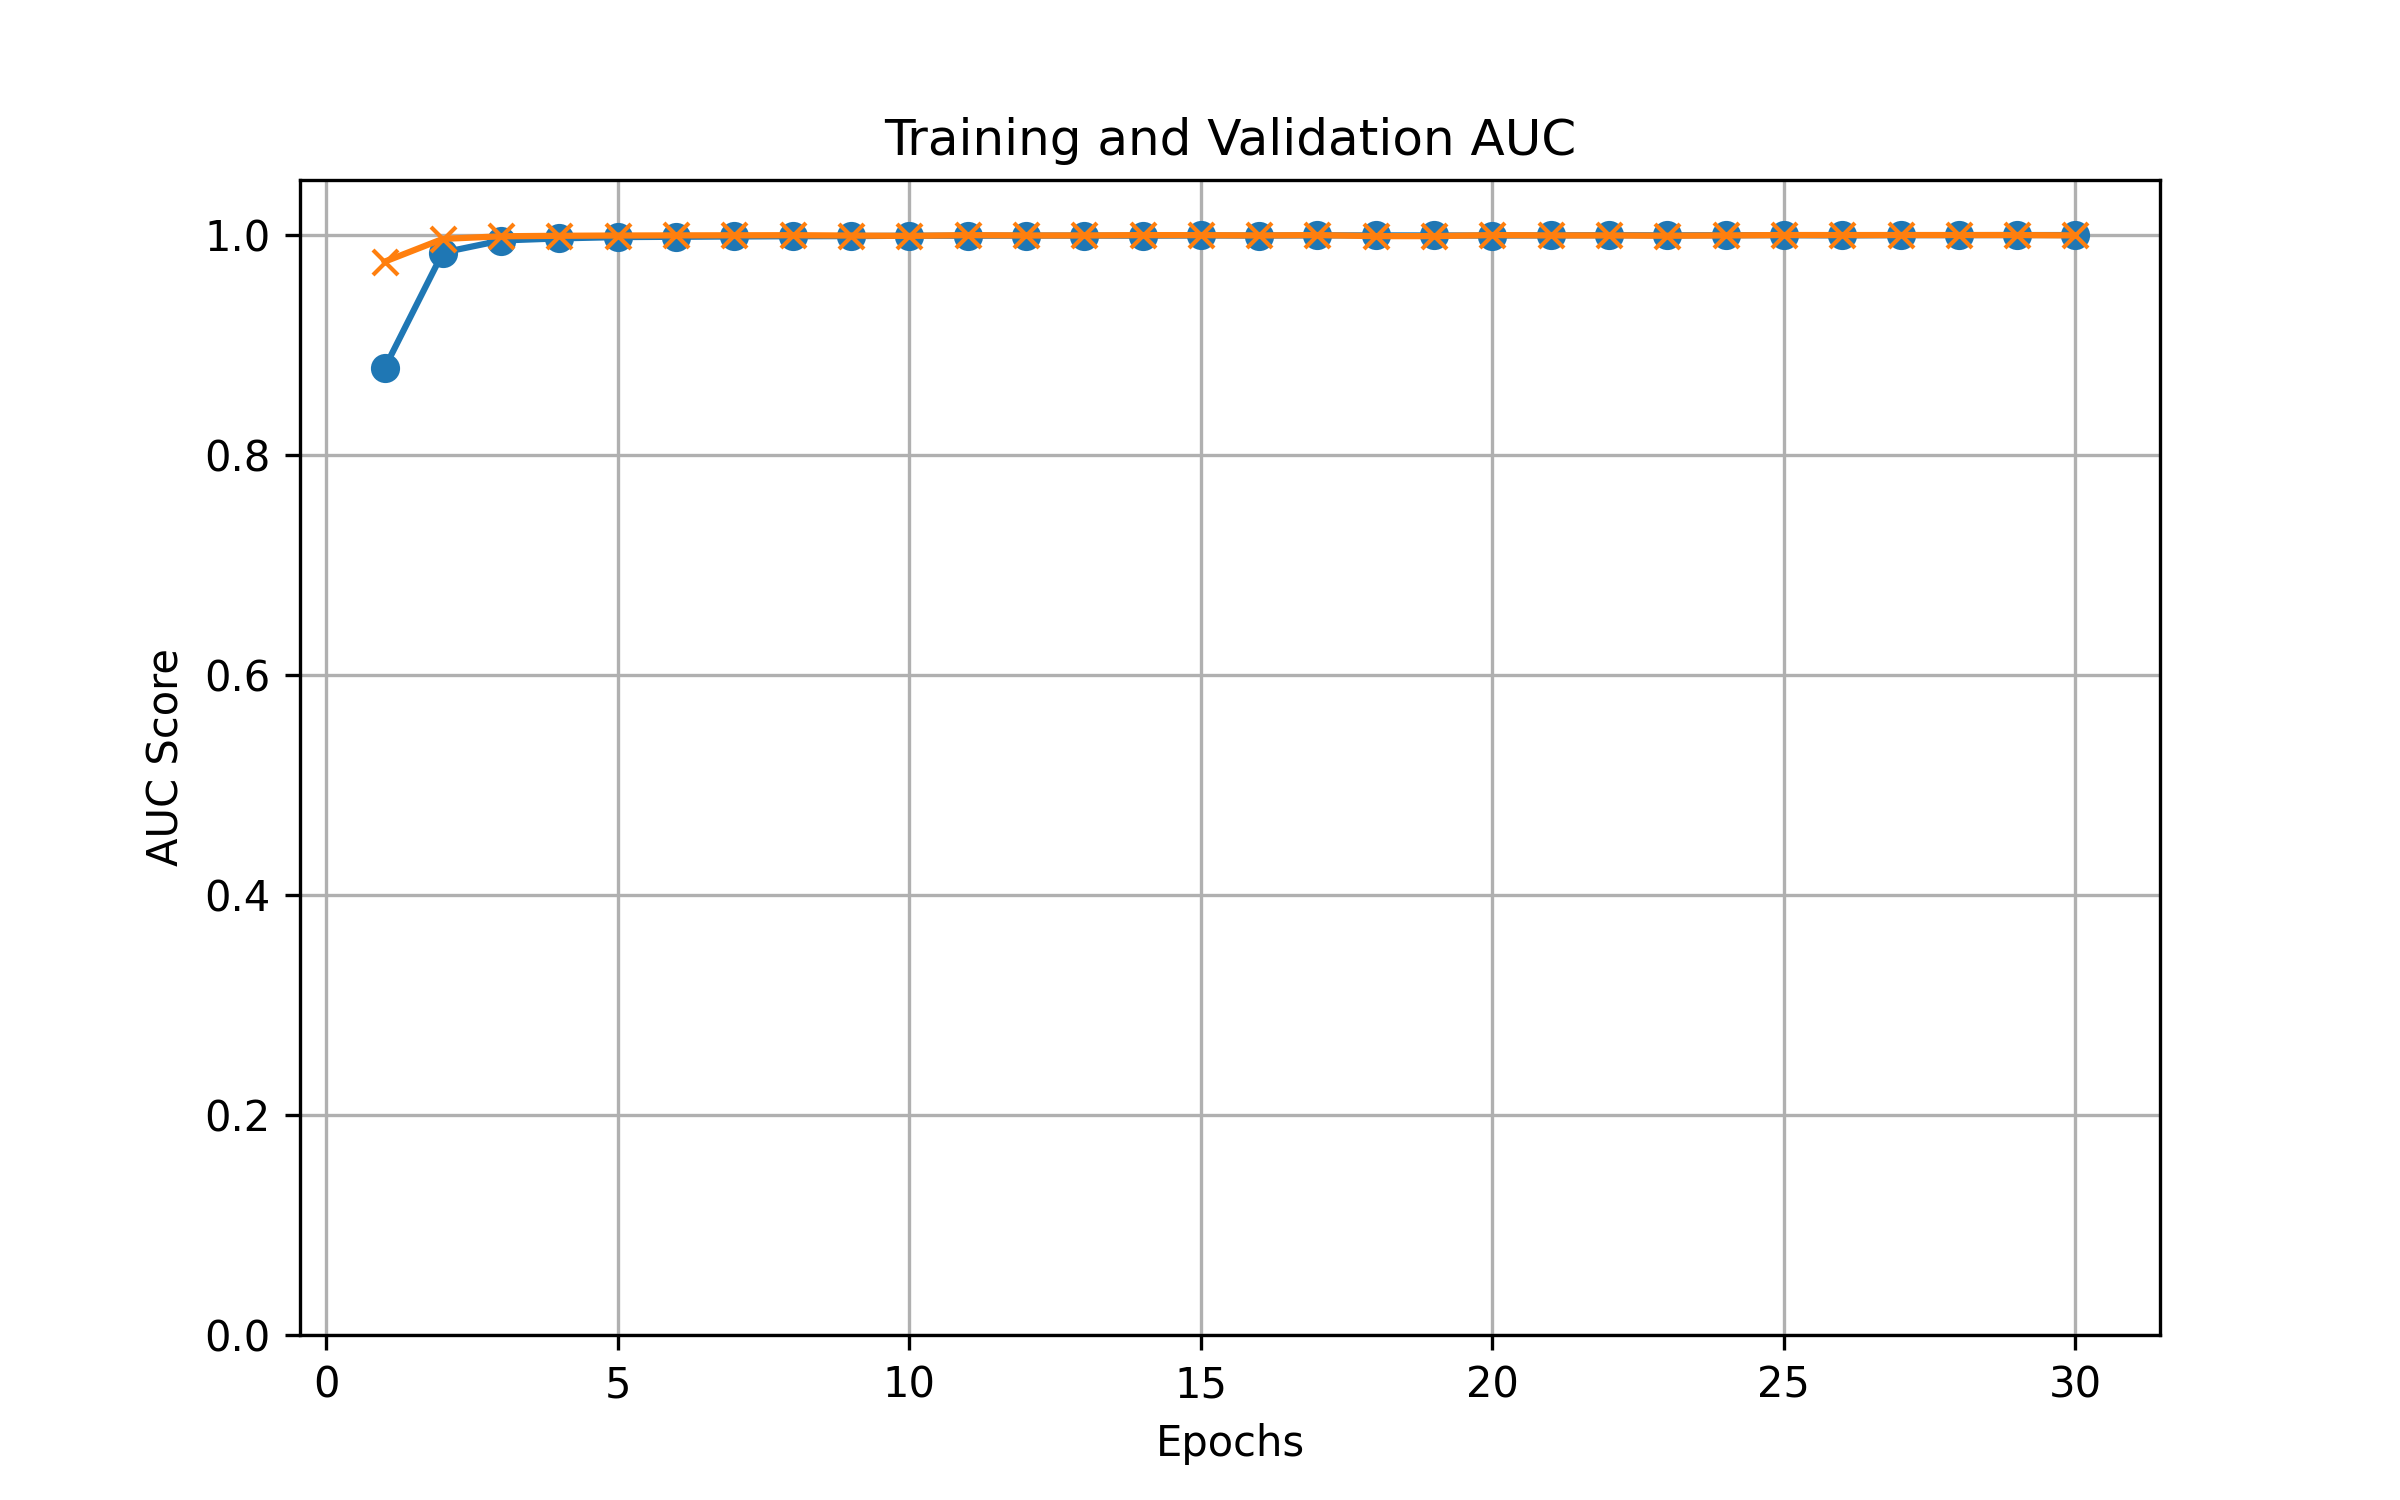
\includegraphics[width=0.47\textwidth]{figures/xception_auc.png}
}
\caption{Training and validation AUC curves for the evaluated models. (\textbf{a}) InceptionV3. (\textbf{b}) MobileNetV2. (\textbf{c}) MobileNetV2 + CBAM. (\textbf{d}) Xception. The AUC curves provide additional evidence of the discriminative capability of each model across training epochs.}
\label{fig:training_validation_auc}
\end{figure}

\begin{figure}[H]
\centering
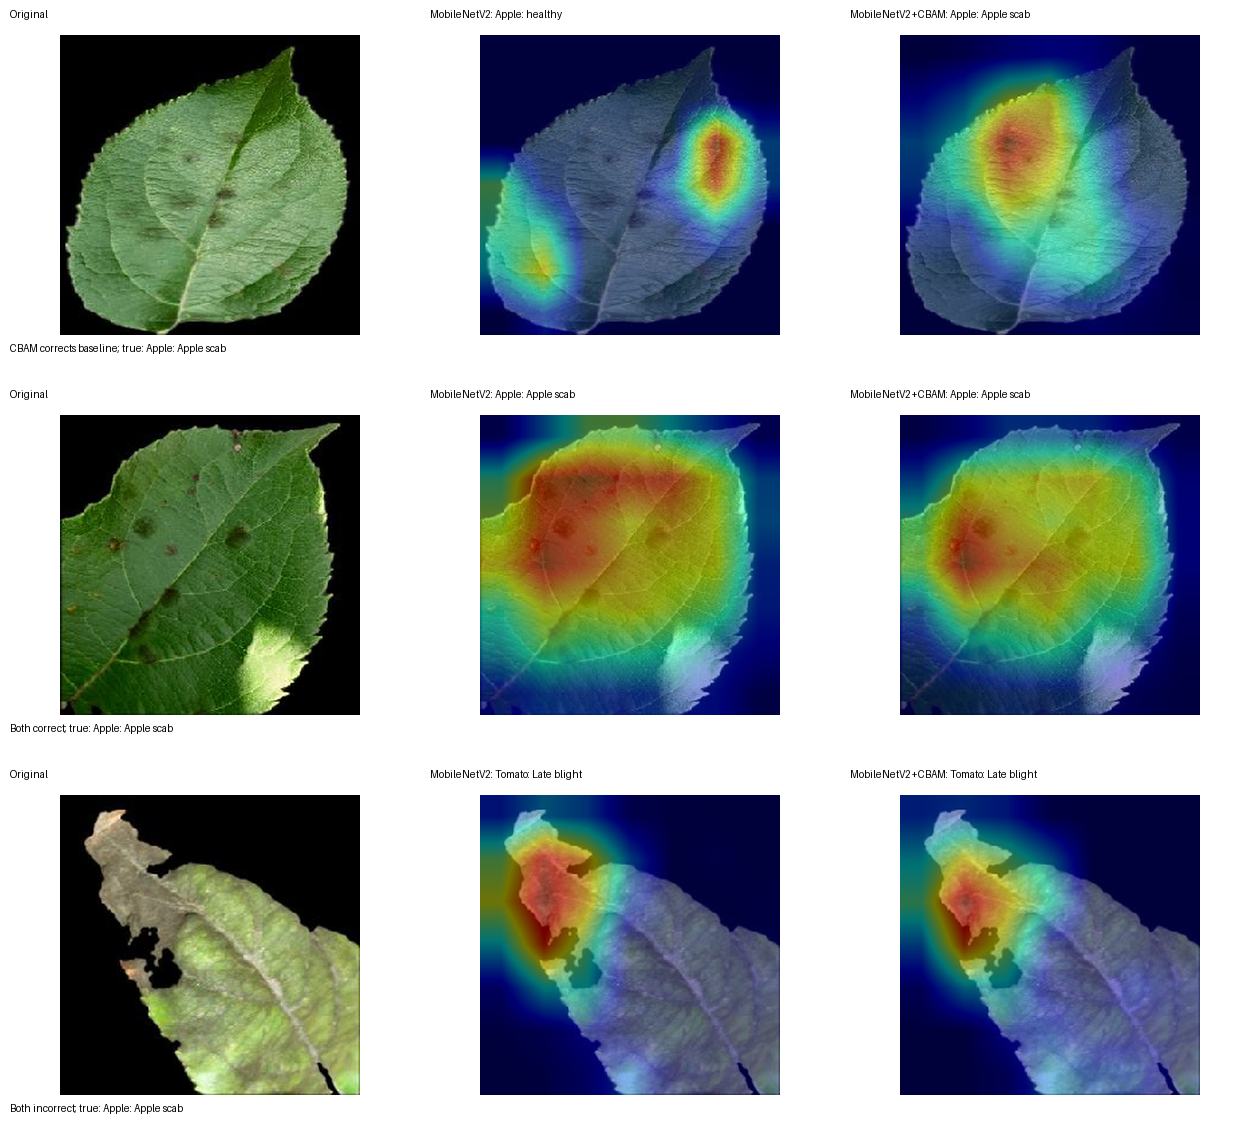
\includegraphics[width=\textwidth]{figures/gradcam_baseline_vs_cbam.png}
\caption{Matched Grad-CAM comparison for MobileNetV2 and MobileNetV2 + CBAM. The first row shows a sample misclassified as healthy by MobileNetV2 but correctly classified as apple scab by the CBAM model. The second row is correctly classified by both models. The third row is misclassified by both models as tomato late blight, illustrating that attention localization does not guarantee class-specific discrimination.}
\label{fig:gradcam_comparison}
\end{figure}

The training curves indicate that the evaluated models converged within the training period. Figure~\ref{fig:gradcam_comparison} provides qualitative evidence about feature localization. In the first example, CBAM shifts the strongest response toward a broader central leaf region and corrects the baseline prediction. In the second example, both models attend to visible scab regions. In the failure example, both concentrate on the damaged leaf apex but predict the wrong disease class. The visualization therefore supports lesion-sensitive behavior in selected cases while also showing that CBAM does not consistently resolve symptom ambiguity.

Taken together, the single-training-run results show a small improvement over MobileNetV2. On the independently converted TensorFlow Lite models, CBAM improved paired test accuracy by 0.64 percentage points (95\% CI: 0.31--0.96); it uniquely corrected 117 samples while MobileNetV2 uniquely corrected 65 (exact two-sided McNemar $p=1.42\times10^{-4}$). This paired test indicates that the observed prediction difference is unlikely to arise from test-sample variation alone, but it does not replace mean $\pm$ standard deviation over independently trained seeds.

\subsection{Deployment and Computational Analysis}

Beyond classification accuracy, deployment-oriented assessment requires reproducible complexity, storage, quantized accuracy, and latency measurements. Table~\ref{tab:deployment_comparison} reports graph-level FLOPs and approximate MACs together with exact serialized sizes and the standardized laptop-CPU benchmark.

\begin{table}[H]
\caption{Computational and CPU deployment comparison. Latency is TensorFlow Lite/XNNPACK, eight CPU threads, batch size one, 50 warm-up and 200 timed runs; preprocessing is excluded. TFLite sizes use MiB ($2^{20}$ bytes).}
\label{tab:deployment_comparison}
\centering
\small
\begin{tabularx}{\textwidth}{l c c c c c}
\toprule
\textbf{Model} & \textbf{Params} & \textbf{GFLOPs} & \textbf{TFLite} & \textbf{Median} & \textbf{P95} \\
\midrule
InceptionV3 & 23.94 M & 11.451 & 23.10 MiB & 10.71 ms & 12.27 ms \\
MobileNetV2 & 3.61 M & 0.602 & 3.68 MiB & 45.38 ms & 106.96 ms \\
MobileNetV2 + CBAM & 4.02 M & 0.604 & 4.07 MiB & 45.42 ms & 102.54 ms \\
Xception & 23.00 M & 9.115 & 22.57 MiB & 200.15 ms & 304.13 ms \\
\bottomrule
\end{tabularx}
\normalsize
\end{table}

CBAM adds 409,699 parameters to MobileNetV2 but only 0.0019 GFLOPs (approximately 0.0010 GMACs) because it is applied once to the final $7\times7$ feature map. The H5/TFLite sizes are 36.26/3.68 MiB for MobileNetV2 and 40.98/4.07 MiB for MobileNetV2 + CBAM. Median CPU latency differs by only 0.05 ms in this XNNPACK benchmark, although both MobileNet variants show substantial scheduling variability at the 95th percentile. Xception remains the most accurate model but is approximately 5.7 times larger than the CBAM TFLite file and requires 15 times its approximate MACs.

The converter used \texttt{Optimize.DEFAULT} without a representative calibration dataset. This is dynamic-range weight quantization: model inputs and outputs remain float32 while eligible weights are quantized at runtime. Table~\ref{tab:quantized_accuracy} shows that conversion preserved most classification performance. The largest reduction was 0.71 percentage points for MobileNetV2, while MobileNetV2 + CBAM decreased by 0.47 points.

\begin{table}[H]
\caption{Floating-point H5 and dynamic-range TFLite test performance. Weighted F1 and macro one-vs-rest AUC are shown for the TFLite models.}
\label{tab:quantized_accuracy}
\centering
\small
\begin{tabularx}{\textwidth}{l c c c c c}
\toprule
\textbf{Model} & \textbf{H5 Acc.} & \textbf{TFLite Acc.} & \textbf{$\Delta$ Acc.} & \textbf{TFLite F1} & \textbf{TFLite AUC} \\
\midrule
InceptionV3 & 96.89\% & 96.80\% & $-$0.09 pp & 96.80\% & 99.96\% \\
MobileNetV2 & 96.78\% & 96.07\% & $-$0.71 pp & 96.07\% & 99.96\% \\
MobileNetV2 + CBAM & 97.17\% & 96.70\% & $-$0.47 pp & 96.69\% & 99.96\% \\
Xception & 98.30\% & 98.22\% & $-$0.07 pp & 98.23\% & 99.98\% \\
\bottomrule
\end{tabularx}
\normalsize
\end{table}

Excluding the seven test images with an exact duplicate in another split changed TFLite accuracy by less than 0.01 percentage points for every model (e.g., 96.70\% to 96.70\% for MobileNetV2 + CBAM after rounding). Thus, the detected exact duplicates do not explain the reported ranking, although future split generation should group duplicate content before partitioning.

Overall, MobileNetV2 + CBAM is compact and slightly more accurate than MobileNetV2, with negligible additional graph operations in this late-placement design. The gain remains modest, plausibly because PlantVillage's uniform backgrounds and salient symptoms leave limited irrelevant content for spatial attention to suppress. Energy consumption was not measured, and a laptop CPU is not a substitute for a target phone, Raspberry Pi, or microcontroller.

\subsection{Limitations and External Validity}

The study evaluates controlled-background image classification. PlantVillage does not capture field clutter, illumination changes, partial leaves, occlusion, overlapping foliage, camera motion, or heterogeneous symptom severity. Spatial attention may learn acquisition regularities as well as lesions, so the results should not be generalized to field deployment without external validation. The archived pipeline also used only a subset of the nominal training and validation directories and contained 10 exact cross-split duplicate groups; these details have been audited and disclosed, and a duplicate-excluded sensitivity analysis was added. Finally, each architecture represents one training run. The paired McNemar result and confidence interval quantify test-sample uncertainty for the saved models, but not seed-to-seed training variability. Independent reruns, attention-placement/module ablations, and target-device energy measurements remain necessary.



%%%%%%%%%%%%%%%%%%%%%%%%%%%%%%%%%%%%%%%%%%
\section{Conclusion}

This paper presented an attention-enhanced MobileNetV2 framework for plant disease detection on resource-constrained devices. The proposed model integrates the Convolutional Block Attention Module (CBAM) after the final MobileNetV2 feature map and before global average pooling, enabling sequential channel and spatial attention to refine extracted features while preserving a lightweight architecture.

Experiments used 54,306 PlantVillage images across 38 classes. In the consistent saved-model re-evaluation, MobileNetV2 + CBAM achieved 97.17\% accuracy and 97.15\% weighted F1-score, compared with 96.78\% and 96.73\% for MobileNetV2. Xception remained most accurate at 98.30\%. A matched Grad-CAM analysis showed examples in which CBAM broadened lesion-focused activation and corrected a baseline error, but also a shared failure in which both models attended to damaged tissue and predicted the wrong disease.

MobileNetV2 + CBAM contains 4.02 million parameters, requires 0.604 GFLOPs (approximately 0.302 GMACs), and converts to a 4.07 MiB dynamic-range-quantized TFLite file. Quantized accuracy was 96.70\%, a 0.47-percentage-point decrease from the re-evaluated H5 model. On an Intel i7-11800H CPU with TFLite/XNNPACK and eight threads, its median batch-one latency was 45.42 ms (P95: 102.54 ms), essentially equal to MobileNetV2 under the same protocol. These measurements establish a platform-specific compactness result rather than universal real-time readiness.

The conclusions remain limited by controlled-background data, the legacy generator subsampling, 10 audited exact cross-split duplicate groups, and the absence of independently trained seeds. Removing the seven duplicated test images had a negligible effect, but future splits should group duplicate content before partitioning. The study also does not establish robustness to field clutter, illumination, occlusion, symptom severity, or domain shift. No phone, Raspberry Pi, microcontroller, or energy benchmark was performed. Future work should report mean $\pm$ standard deviation across seeds, compare unfreezing depths and CBAM placements, test SE/ECA/coordinate attention and modern lightweight backbones, validate on field datasets, and measure latency, peak memory, and energy on representative target hardware.


%%%%%%%%%%%%%%%%%%%%%%%%%%%%%%%%%%%%%%%%%%
\vspace{6pt} 

%%%%%%%%%%%%%%%%%%%%%%%%%%%%%%%%%%%%%%%%%%
%% optional
%\supplementary{The following supporting information can be downloaded at:  \linksupplementary{s1}, Figure S1: title; Table S1: title; Video S1: title.}

% Only for journal Methods and Protocols:
% If you wish to submit a video article, please do so with any other supplementary material.
% \supplementary{The following supporting information can be downloaded at: \linksupplementary{s1}, Figure S1: title; Table S1: title; Video S1: title. A supporting video article is available at doi: link.}

% Only used for preprtints:
% \supplementary{The following supporting information can be downloaded at the website of this paper posted on \href{https://www.preprints.org/}{Preprints.org}.}

% Only for journal Hardware:
% If you wish to submit a video article, please do so with any other supplementary material.
% \supplementary{The following supporting information can be downloaded at: \linksupplementary{s1}, Figure S1: title; Table S1: title; Video S1: title.\vspace{6pt}\\
%\begin{tabularx}{\textwidth}{lll}
%\toprule
%\textbf{Name} & \textbf{Type} & \textbf{Description} \\
%\midrule
%S1 & Python script (.py) & Script of python source code used in XX \\
%S2 & Text (.txt) & Script of modelling code used to make Figure X \\
%S3 & Text (.txt) & Raw data from experiment X \\
%S4 & Video (.mp4) & Video demonstrating the hardware in use \\
%... & ... & ... \\
%\bottomrule
%\end{tabularx}
%}

%%%%%%%%%%%%%%%%%%%%%%%%%%%%%%%%%%%%%%%%%%
\authorcontributions{
Conceptualization, E.U., M.A.A.M. and M.A.; methodology, E.U., M.A.A.M. and M.A.; software, E.U.; validation, E.U., M.A.A.M. and M.A.; formal analysis, E.U.; investigation, E.U.; resources, E.U.; data curation, E.U.; writing---original draft preparation, E.U.; writing---review and editing, E.U., M.A.A.M. and M.A.; visualization, E.U.; supervision, M.A.A.M. and M.A.; project administration, M.A.A.M. and M.A. All authors have read and agreed to the published version of the manuscript.
}

\funding{
This research received no external funding.
}

\institutionalreview{
Not applicable.
}

\informedconsent{
Not applicable.
}

\dataavailability{
The PlantVillage dataset is publicly available. The train/validation/test split script, training notebooks, saved H5 and TensorFlow Lite models, dataset-audit manifest, evaluation scripts, and derived analysis outputs will be deposited in a permanent public repository; the archival URL/DOI will be inserted before publication.
}

\acknowledgments{
The authors would like to acknowledge the Department of Computer Science at Bishop's University for providing academic support during this research work.
}

\conflictsofinterest{
The authors declare no conflicts of interest.
}

%%%%%%%%%%%%%%%%%%%%%%%%%%%%%%%%%%%%%%%%%%
\abbreviations{Abbreviations}{
The following abbreviations are used in this manuscript:
\\

\noindent
\begin{tabular}{@{}ll}
AUC & Area Under the Curve\\
CBAM & Convolutional Block Attention Module\\
CNN & Convolutional Neural Network\\
GAP & Global Average Pooling\\
GPU & Graphics Processing Unit\\
MLP & Multilayer Perceptron\\
TFLite & TensorFlow Lite\\
\end{tabular}
}

%%%%%%%%%%%%%%%%%%%%%%%%%%%%%%%%%%%%%%%%%%
%\isPreprints{}{% This command is only used for ``preprints''.
\begin{adjustwidth}{-\extralength}{0cm}
%} % If the paper is ``preprints'', please uncomment this parenthesis.

\reftitle{References}

\bibliography{references}

%%%%%%%%%%%%%%%%%%%%%%%%%%%%%%%%%%%%%%%%%%
\PublishersNote{}
%\isPreprints{}{% This command is only used for ``preprints''.
\end{adjustwidth}
%} % If the paper is ``preprints'', please uncomment this parenthesis.

\end{document}
